\PassOptionsToPackage{unicode=true}{hyperref} % options for packages loaded elsewhere
\PassOptionsToPackage{hyphens}{url}
%
\documentclass[
]{book}
\usepackage{lmodern}
\usepackage{amssymb,amsmath}
\usepackage{ifxetex,ifluatex}
\ifnum 0\ifxetex 1\fi\ifluatex 1\fi=0 % if pdftex
  \usepackage[T1]{fontenc}
  \usepackage[utf8]{inputenc}
  \usepackage{textcomp} % provides euro and other symbols
\else % if luatex or xelatex
  \usepackage{unicode-math}
  \defaultfontfeatures{Scale=MatchLowercase}
  \defaultfontfeatures[\rmfamily]{Ligatures=TeX,Scale=1}
\fi
% use upquote if available, for straight quotes in verbatim environments
\IfFileExists{upquote.sty}{\usepackage{upquote}}{}
\IfFileExists{microtype.sty}{% use microtype if available
  \usepackage[]{microtype}
  \UseMicrotypeSet[protrusion]{basicmath} % disable protrusion for tt fonts
}{}
\makeatletter
\@ifundefined{KOMAClassName}{% if non-KOMA class
  \IfFileExists{parskip.sty}{%
    \usepackage{parskip}
  }{% else
    \setlength{\parindent}{0pt}
    \setlength{\parskip}{6pt plus 2pt minus 1pt}}
}{% if KOMA class
  \KOMAoptions{parskip=half}}
\makeatother
\usepackage{xcolor}
\IfFileExists{xurl.sty}{\usepackage{xurl}}{} % add URL line breaks if available
\IfFileExists{bookmark.sty}{\usepackage{bookmark}}{\usepackage{hyperref}}
\hypersetup{
  pdftitle={Métodos quantitativos em Psicologia com R e Rstudio},
  pdfauthor={Luis Anunciação (PUC-Rio), PhD},
  pdfborder={0 0 0},
  breaklinks=true}
\urlstyle{same}  % don't use monospace font for urls
\usepackage{color}
\usepackage{fancyvrb}
\newcommand{\VerbBar}{|}
\newcommand{\VERB}{\Verb[commandchars=\\\{\}]}
\DefineVerbatimEnvironment{Highlighting}{Verbatim}{commandchars=\\\{\}}
% Add ',fontsize=\small' for more characters per line
\usepackage{framed}
\definecolor{shadecolor}{RGB}{248,248,248}
\newenvironment{Shaded}{\begin{snugshade}}{\end{snugshade}}
\newcommand{\AlertTok}[1]{\textcolor[rgb]{0.94,0.16,0.16}{#1}}
\newcommand{\AnnotationTok}[1]{\textcolor[rgb]{0.56,0.35,0.01}{\textbf{\textit{#1}}}}
\newcommand{\AttributeTok}[1]{\textcolor[rgb]{0.77,0.63,0.00}{#1}}
\newcommand{\BaseNTok}[1]{\textcolor[rgb]{0.00,0.00,0.81}{#1}}
\newcommand{\BuiltInTok}[1]{#1}
\newcommand{\CharTok}[1]{\textcolor[rgb]{0.31,0.60,0.02}{#1}}
\newcommand{\CommentTok}[1]{\textcolor[rgb]{0.56,0.35,0.01}{\textit{#1}}}
\newcommand{\CommentVarTok}[1]{\textcolor[rgb]{0.56,0.35,0.01}{\textbf{\textit{#1}}}}
\newcommand{\ConstantTok}[1]{\textcolor[rgb]{0.00,0.00,0.00}{#1}}
\newcommand{\ControlFlowTok}[1]{\textcolor[rgb]{0.13,0.29,0.53}{\textbf{#1}}}
\newcommand{\DataTypeTok}[1]{\textcolor[rgb]{0.13,0.29,0.53}{#1}}
\newcommand{\DecValTok}[1]{\textcolor[rgb]{0.00,0.00,0.81}{#1}}
\newcommand{\DocumentationTok}[1]{\textcolor[rgb]{0.56,0.35,0.01}{\textbf{\textit{#1}}}}
\newcommand{\ErrorTok}[1]{\textcolor[rgb]{0.64,0.00,0.00}{\textbf{#1}}}
\newcommand{\ExtensionTok}[1]{#1}
\newcommand{\FloatTok}[1]{\textcolor[rgb]{0.00,0.00,0.81}{#1}}
\newcommand{\FunctionTok}[1]{\textcolor[rgb]{0.00,0.00,0.00}{#1}}
\newcommand{\ImportTok}[1]{#1}
\newcommand{\InformationTok}[1]{\textcolor[rgb]{0.56,0.35,0.01}{\textbf{\textit{#1}}}}
\newcommand{\KeywordTok}[1]{\textcolor[rgb]{0.13,0.29,0.53}{\textbf{#1}}}
\newcommand{\NormalTok}[1]{#1}
\newcommand{\OperatorTok}[1]{\textcolor[rgb]{0.81,0.36,0.00}{\textbf{#1}}}
\newcommand{\OtherTok}[1]{\textcolor[rgb]{0.56,0.35,0.01}{#1}}
\newcommand{\PreprocessorTok}[1]{\textcolor[rgb]{0.56,0.35,0.01}{\textit{#1}}}
\newcommand{\RegionMarkerTok}[1]{#1}
\newcommand{\SpecialCharTok}[1]{\textcolor[rgb]{0.00,0.00,0.00}{#1}}
\newcommand{\SpecialStringTok}[1]{\textcolor[rgb]{0.31,0.60,0.02}{#1}}
\newcommand{\StringTok}[1]{\textcolor[rgb]{0.31,0.60,0.02}{#1}}
\newcommand{\VariableTok}[1]{\textcolor[rgb]{0.00,0.00,0.00}{#1}}
\newcommand{\VerbatimStringTok}[1]{\textcolor[rgb]{0.31,0.60,0.02}{#1}}
\newcommand{\WarningTok}[1]{\textcolor[rgb]{0.56,0.35,0.01}{\textbf{\textit{#1}}}}
\usepackage{longtable,booktabs}
% Allow footnotes in longtable head/foot
\IfFileExists{footnotehyper.sty}{\usepackage{footnotehyper}}{\usepackage{footnote}}
\makesavenoteenv{longtable}
\usepackage{graphicx,grffile}
\makeatletter
\def\maxwidth{\ifdim\Gin@nat@width>\linewidth\linewidth\else\Gin@nat@width\fi}
\def\maxheight{\ifdim\Gin@nat@height>\textheight\textheight\else\Gin@nat@height\fi}
\makeatother
% Scale images if necessary, so that they will not overflow the page
% margins by default, and it is still possible to overwrite the defaults
% using explicit options in \includegraphics[width, height, ...]{}
\setkeys{Gin}{width=\maxwidth,height=\maxheight,keepaspectratio}
\setlength{\emergencystretch}{3em}  % prevent overfull lines
\providecommand{\tightlist}{%
  \setlength{\itemsep}{0pt}\setlength{\parskip}{0pt}}
\setcounter{secnumdepth}{5}
% Redefines (sub)paragraphs to behave more like sections
\ifx\paragraph\undefined\else
  \let\oldparagraph\paragraph
  \renewcommand{\paragraph}[1]{\oldparagraph{#1}\mbox{}}
\fi
\ifx\subparagraph\undefined\else
  \let\oldsubparagraph\subparagraph
  \renewcommand{\subparagraph}[1]{\oldsubparagraph{#1}\mbox{}}
\fi

% set default figure placement to htbp
\makeatletter
\def\fps@figure{htbp}
\makeatother

\usepackage{booktabs}
\usepackage{amsthm}
\makeatletter
\def\thm@space@setup{%
  \thm@preskip=8pt plus 2pt minus 4pt
  \thm@postskip=\thm@preskip
}
\makeatother
\usepackage[]{natbib}
\bibliographystyle{apalike}

\title{Métodos quantitativos em Psicologia com R e Rstudio}
\author{\href{mailto:\%20luisfca@gmail.com}{Luis Anunciação (PUC-Rio), PhD}}
\date{2020-03-28}

\begin{document}
\maketitle

{
\setcounter{tocdepth}{1}
\tableofcontents
}
\hypertarget{introduuxe7uxe3o}{%
\chapter{Introdução}\label{introduuxe7uxe3o}}

Aprender estatística e análise de dados é uma das tarefas mais importantes e desafiadoras que existe no meio acadêmico, especialmente às disciplinas agrupadas em ciências humanas, como Psicologia. Por consequência, ensinar ambas as matérias também impõe um desafio enorme, mas necessário.

Por diversas razões, as pesquisas feitas em Psicologia apresentam muitas informações misturadas e sobrepostas e a utilização da estatística é fundamental para conseguir separar e filtrar àquelas informações que temos interesse (sinal) daquelas que apenas distorcem estas primeiras (ruído).

\hypertarget{estatuxedstica-descritiva}{%
\chapter{Estatística Descritiva}\label{estatuxedstica-descritiva}}

\begin{objectives}
\textbf{Objetivos do capítulo}\\
1. Apresentar os verbos do dplyr e funções do ggplot.\\
2. Revisitar conceitos básicos de estatística descritiva\\
3. Ensinar a construção de tabelas e gráficos
\end{objectives}

Base usada: Dados - Brasil e espanha fusionados
AFONSO JR, ARMANDO ; PORTUGAL, A. C. A. ; SANTOS, E. J. R. ; BULLON, F. F. ; VILHENA, J. ; ANUNCIAÇÃO, LUIS . Sintomas de depressão e ansiedade em universitários espanhóis, portugueses e brasileiros. PSICOLOGIA: TEORIA E PESQUISA (UNB. IMPRESSO), 2020.

A apresentação dos resultados de uma pesquisa a partir de gráficos e tabelas é fundamental para disseminação dos achados tanto entre pares acadêmicos como para sociedade em geral. No geral, o R e seus pacotes oferecem excelentes ferramentas para aspectos descritivos. No entanto, algumas apresentações relativamente simples trazem uma dificuldade computacional, o que pode gerar alguma desvantagem na utilização do R para tais apresentações quando comparados com programas mais acessíveis, como o Excel. Apesar dessa condição, a relação entre dificuldade e complexidade favorece o R àquelas tarefas mais complicadas, como realizar análises inferenciais e psicométricas, como apresentado a seguir.

\begin{figure}
\centering
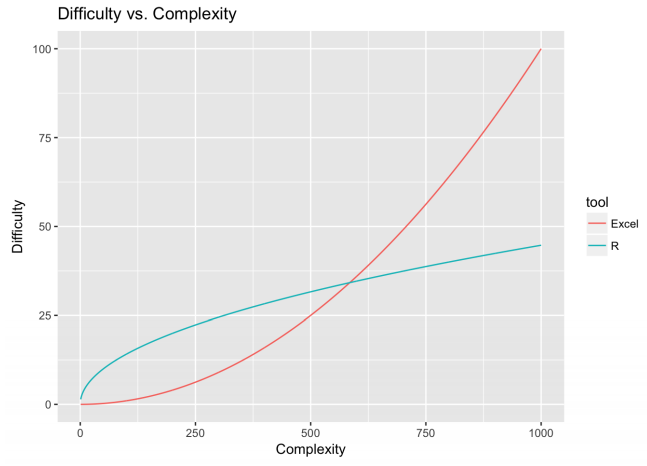
\includegraphics{./img/excel_r.PNG}
\caption{Excel vs R}
\end{figure}

Posto isso, todo resultado estatístico começa pela apresentação de \textbf{tabelas} e \textbf{gráficos}. Da mesma forma que a construção de um prédio depende que andaimes sejam colocados, um relatório técnico depende dessas condições. Aproveitando um pouco mais esse exemplo, da mesma maneira que a conclusão da construção de um prédio, necessariamente, cursa com a retirada dos andaimes, artigos científicos frequentemente tem espaço limitado para publicação e, consequentemente, os autores se veem na situação de aproveitar apenas parte (ou quase nada) dos relatórios originais.

\hypertarget{pesquisa}{%
\section{Pesquisa}\label{pesquisa}}

Vamos utilizar a pesquisa intitulada ``Sintomas de depressão e ansiedade em universitários espanhóis, portugueses e brasileiros'', com previsão de publicação pela Revista Psicologia: Teoria e Pesquisa em 2019. Nessa pesquisa, sou o coautor e o pesquisador responsável para correspondência.

O objetivo dessa pesquisa foi explorar sintomas de ansiedade e depressão em universitários, bem como investigar possíveis relações entre tais traços latentes e fatores sociodemográficos. Um diferencial importante dessa pesquisa foi a seleção amostral. Partiu-se de uma amostra representativa dos estudantes de três universidades, PUC-Rio (Brasil), Universidade de Extremadura (Espanha) e Universidade de Coimbra (Portugal). Isso permitiu ter maior validade externa dos resultados.

Todo documento acadêmico e científico é composto de \textbf{aspectos textuais}, \textbf{aspectos tabulares} e \textbf{gráficos} que devem caminhar na mesma direção e \textbf{sempre associados às perguntas e objetivos traçados na pesquisa}. Assim, é possível concluir que a parte principal de qualquer trabalho acadêmico não é necessariamente os aspectos estatísticos, mas sim os objetivos e possíveis hipóteses investigadas pelos pesquisadores. A estatística é uma ferramenta de trabalho (ou uma atividade de meio) para que as perguntas sejam respondidas de forma válida.

Conforme já explicitado, a estatística pode ser dividida em duas áreas interligadas: estatística descritiva e estatística inferencial. O objetivo da estatística descritiva é apresentar sínteses e resumos dos resultados a partir de gráficos e tabelas. Não é intenção dessa área fazer generalizações ou extrapolar os resultados obtidos em uma pesquisa a pessoas não investigadas durante a coleta de dados. Por contraste, a estatística inferencial visa extrapolar os dados e fazer generalizações que toquem toda população de onde aquela mostra foi retirada e é representativa. Dessa maneira, o principal objetivo da estatística inferencial é, de fato, fazer inferências.

Apesar de livros e aulas unirem ambas as áreas da estatística, alguns pontos merecem destaque, que são:

\begin{enumerate}
\def\labelenumi{\arabic{enumi}.}
\item
  A estatística descritiva surgiu antes que a inferencial. A etimologia da palavra talvez ajude a entender, uma vez que estatística vem da palavra estado e este sempre teve interesse em saber quantos eram os cidadãos de um determinado local para, entre outras atividades, taxá-los. Dessa maneira, aspectos descritivos antecedem os inferenciais. Por sua vez, a estatística inferencial guarda origem e proximidade com a teoria dos jogos e, consequentemente, isso ajuda a entender o motivo pelo qual a maioria dos exemplos inferenciais envolvem jogos de azar.
\item
  A estatística tem duas ``escolas'' ou ``formas de pensamento''. A estatística frequentista e a estatística bayesiana. Aspectos fundamentais que tocam à definição de probabilidade são diferentes, bem como a definição de dados e parâmetros também o são. Pela perspectiva histórica, a estatística bayesiana é mais antiga que a frequentista. No entanto, se for comparado a proporção de uso entre os pesquisadores, a estatística frequentista é ainda a mais frequente e justifica a ênfase deste livro nesta área.
\item
  A relação entre estatística e Machine Learning (ML) é relativamente recente. Apesar de grande interface, e do fato que as análises realizadas em estatística e ML encontram resultados virtualmente idênticos, as áreas têm objetivos diferentes. Ainda sob perspectiva histórica, a estatística, como uma área do conhecimento, é anterior à ML e, também por isso, justifica a ênfase do livro.
\end{enumerate}

\hypertarget{verbos-do-dplyr}{%
\section{Verbos do dplyr}\label{verbos-do-dplyr}}

O dplyr funciona de maneira muito intuitiva. O padrão original do R considera que as operações são realizadas a partir de uma lógica do tipo \texttt{verbo(sujeito,\ complemento)} enquanto o ambiente tidyverse opta por \texttt{sujeito\ \%\textgreater{}\%\ verbo(complemento)}, tornando-se o ato de programar mais natural e associado à maneira que organizamos as ideias.

Os verbos principais do pacote estão listados na tabela a seguir e as sintaxes deixadas no decorrer deste capítulo (e do livro) permitem uma melhor apreensão das funcionalidades. É importante lembrar que, em alguns momentos, em função da praticidade computacional, algumas sintaxes vão contar com o formato base do R.

\begin{longtable}[]{@{}lc@{}}
\toprule
Verbo & Ação\tabularnewline
\midrule
\endhead
glimpse & Inspeciona os dados\tabularnewline
count & Conta os níveis de uma variável\tabularnewline
select & seleciona uma variável específica\tabularnewline
filter & Filtra os resultados por um nível específico de uma variável\tabularnewline
group\_by & Agrupa os resultados por níveis de uma variávei específica\tabularnewline
summarise & Apresenta sumários (com medidas estatísticas)\tabularnewline
mutate & Cria novas variáveis ou altera as existentes\tabularnewline
arrange & Organiza a apresentação dos resultados\tabularnewline
left\_join & Junta bases ou colunas\tabularnewline
gather & Transforma uma base larga em longa\tabularnewline
spread & Transforma uma base longa em larga\tabularnewline
\bottomrule
\end{longtable}

\hypertarget{tabelas}{%
\section{Tabelas}\label{tabelas}}

Tabelas apresentam as informações de uma pesquisa de maneira reunida e objetiva. Como os verbos do dplyr possibilitam que os mesmos resultados sejam encontrados por vias diferentes, os códigos a seguir tentarão manter uma uniformidade lógica. Em alguns momentos, para ampliar as possibilidades de codificação, sintaxes extras serão oferecidas.

A tabela a seguir apresenta a quantidade de participantes em cada país.

\begin{Shaded}
\begin{Highlighting}[]
\NormalTok{Dataset }\OperatorTok\StringTok{ }
\StringTok{  }\KeywordTok{group_by}\NormalTok{(country) }\OperatorTok\StringTok{ }
\StringTok{  }\KeywordTok{summarise}\NormalTok{(}\DataTypeTok{n=}\KeywordTok{n}\NormalTok{()) }\OperatorTok\StringTok{ }
\StringTok{  }\KeywordTok{kable}\NormalTok{(}\DataTypeTok{digits =} \DecValTok{2}\NormalTok{) }\OperatorTok\StringTok{ }
\StringTok{  }\KeywordTok{kable_styling}\NormalTok{(}\DataTypeTok{bootstrap_options =} \KeywordTok{c}\NormalTok{(}\StringTok{"striped"}\NormalTok{, }\StringTok{"hover"}\NormalTok{, }\StringTok{"condensed"}\NormalTok{))}
\end{Highlighting}
\end{Shaded}

country

n

Espanha

1216

Portugal

426

Brasil

315

É também possível adicionar proporções relativas à tabela, o que é uma escolha adequada para apresentação dos resultados.

\begin{Shaded}
\begin{Highlighting}[]
\NormalTok{Dataset }\OperatorTok\StringTok{ }
\StringTok{  }\KeywordTok{group_by}\NormalTok{(country) }\OperatorTok\StringTok{ }
\StringTok{  }\KeywordTok{summarise}\NormalTok{(}\DataTypeTok{n=}\KeywordTok{n}\NormalTok{(), }\DataTypeTok{Prop =}\NormalTok{ n}\OperatorTok{/}\KeywordTok{nrow}\NormalTok{(.)) }\OperatorTok\StringTok{ }
\StringTok{  }\KeywordTok{kable}\NormalTok{(}\DataTypeTok{digits =} \DecValTok{2}\NormalTok{) }\OperatorTok\StringTok{ }
\StringTok{  }\KeywordTok{kable_styling}\NormalTok{(}\DataTypeTok{bootstrap_options =} \KeywordTok{c}\NormalTok{(}\StringTok{"striped"}\NormalTok{, }\StringTok{"hover"}\NormalTok{, }\StringTok{"condensed"}\NormalTok{))}
\end{Highlighting}
\end{Shaded}

country

n

Prop

Espanha

1216

0.62

Portugal

426

0.22

Brasil

315

0.16

O pacote \texttt{janitor} oferece complementos úteis à família tidyverse e um deles justamente adiciona os totais, de maneira mais rápida. Repare que para utilizar o pacote sem tê-lo previamente carregado ao ambiente, basta usar o nome do pacote seguido de ::

\begin{Shaded}
\begin{Highlighting}[]
\NormalTok{Dataset }\OperatorTok\StringTok{ }
\StringTok{  }\KeywordTok{group_by}\NormalTok{(country) }\OperatorTok\StringTok{ }
\StringTok{  }\KeywordTok{summarise}\NormalTok{(}\DataTypeTok{n=}\KeywordTok{n}\NormalTok{(), }\DataTypeTok{prop =}\NormalTok{ n}\OperatorTok{/}\KeywordTok{nrow}\NormalTok{(.)) }\OperatorTok\StringTok{ }
\StringTok{  }\KeywordTok{bind_rows}\NormalTok{(}\KeywordTok{summarise_all}\NormalTok{(., }\KeywordTok{list}\NormalTok{(}\OperatorTok{~}\ControlFlowTok{if}\NormalTok{(}\KeywordTok{is.numeric}\NormalTok{(.)) }\KeywordTok{sum}\NormalTok{(.) }\ControlFlowTok{else} \StringTok{"Total"}\NormalTok{))) }\OperatorTok\StringTok{ }
\StringTok{  }\KeywordTok{kable}\NormalTok{(}\DataTypeTok{digits =} \DecValTok{2}\NormalTok{) }\OperatorTok\StringTok{ }
\StringTok{  }\KeywordTok{kable_styling}\NormalTok{(}\DataTypeTok{bootstrap_options =} \KeywordTok{c}\NormalTok{(}\StringTok{"striped"}\NormalTok{, }\StringTok{"hover"}\NormalTok{, }\StringTok{"condensed"}\NormalTok{))}
\end{Highlighting}
\end{Shaded}

\begin{verbatim}
## Warning in bind_rows_(x, .id): binding factor and character vector,
## coercing into character vector
\end{verbatim}

\begin{verbatim}
## Warning in bind_rows_(x, .id): binding character and factor vector,
## coercing into character vector
\end{verbatim}

country

n

prop

Espanha

1216

0.62

Portugal

426

0.22

Brasil

315

0.16

Total

1957

1.00

\begin{Shaded}
\begin{Highlighting}[]
\NormalTok{Dataset }\OperatorTok\StringTok{ }
\StringTok{  }\KeywordTok{group_by}\NormalTok{(country) }\OperatorTok\StringTok{ }
\StringTok{  }\KeywordTok{summarise}\NormalTok{(}\DataTypeTok{n=}\KeywordTok{n}\NormalTok{(), }\DataTypeTok{prop =}\NormalTok{ n}\OperatorTok{/}\KeywordTok{nrow}\NormalTok{(.)) }\OperatorTok\StringTok{ }
\StringTok{  }\NormalTok{janitor}\OperatorTok{::}\KeywordTok{adorn_totals}\NormalTok{(}\StringTok{"row"}\NormalTok{) }\OperatorTok\StringTok{ }
\StringTok{  }\KeywordTok{kable}\NormalTok{(}\DataTypeTok{digits =} \DecValTok{2}\NormalTok{) }\OperatorTok\StringTok{ }
\StringTok{  }\KeywordTok{kable_styling}\NormalTok{(}\DataTypeTok{bootstrap_options =} \KeywordTok{c}\NormalTok{(}\StringTok{"striped"}\NormalTok{, }\StringTok{"hover"}\NormalTok{, }\StringTok{"condensed"}\NormalTok{))}
\end{Highlighting}
\end{Shaded}

country

n

prop

Espanha

1216

0.62

Portugal

426

0.22

Brasil

315

0.16

Total

1957

1.00

O mesmo que foi realizado com os países, pode também ser realizado com o sexo do participante.

\begin{Shaded}
\begin{Highlighting}[]
\NormalTok{Dataset }\OperatorTok\StringTok{ }
\StringTok{  }\KeywordTok{group_by}\NormalTok{(sex) }\OperatorTok\StringTok{ }
\StringTok{  }\KeywordTok{summarise}\NormalTok{(}\DataTypeTok{n=}\KeywordTok{n}\NormalTok{(), }\DataTypeTok{prop =}\NormalTok{ n}\OperatorTok{/}\KeywordTok{nrow}\NormalTok{(.)) }\OperatorTok\StringTok{ }
\StringTok{  }\NormalTok{janitor}\OperatorTok{::}\KeywordTok{adorn_totals}\NormalTok{(}\StringTok{"row"}\NormalTok{) }\OperatorTok\StringTok{ }
\StringTok{  }\KeywordTok{kable}\NormalTok{(}\DataTypeTok{digits =} \DecValTok{2}\NormalTok{) }\OperatorTok\StringTok{ }
\StringTok{  }\KeywordTok{kable_styling}\NormalTok{(}\DataTypeTok{bootstrap_options =} \KeywordTok{c}\NormalTok{(}\StringTok{"striped"}\NormalTok{, }\StringTok{"hover"}\NormalTok{, }\StringTok{"condensed"}\NormalTok{))}
\end{Highlighting}
\end{Shaded}

\begin{verbatim}
## Warning: Factor `sex` contains implicit NA, consider using
## `forcats::fct_explicit_na`
\end{verbatim}

sex

n

prop

M

736

0.38

F

1214

0.62

NA

7

0.00

Total

1957

1.00

A adição do argumento para filtrar os participantes com dados ausentes sobre sexo auxilia a apresentar melhor os resultados. É importante atentar que essa análise tem finalidade descritiva e que omitir a apresentação de variáveis ausentes não significa excluir ou remover os participantes das análises que serão feitas posteriormente. Somente em possibilidades remotas se retira participantes das análises de maneira definitiva.

\begin{Shaded}
\begin{Highlighting}[]
\NormalTok{Dataset }\OperatorTok\StringTok{ }
\StringTok{  }\KeywordTok{filter}\NormalTok{(}\OperatorTok{!}\KeywordTok{is.na}\NormalTok{(sex)) }\OperatorTok\StringTok{ }
\StringTok{  }\KeywordTok{group_by}\NormalTok{(sex) }\OperatorTok
\StringTok{  }\KeywordTok{summarise}\NormalTok{(}\DataTypeTok{n=}\KeywordTok{n}\NormalTok{(), }\DataTypeTok{prop =}\NormalTok{ n}\OperatorTok{/}\KeywordTok{nrow}\NormalTok{(.)) }\OperatorTok\StringTok{ }
\StringTok{  }\KeywordTok{kable}\NormalTok{(}\DataTypeTok{digits =} \DecValTok{2}\NormalTok{) }\OperatorTok\StringTok{ }
\StringTok{  }\KeywordTok{kable_styling}\NormalTok{(}\DataTypeTok{bootstrap_options =} \KeywordTok{c}\NormalTok{(}\StringTok{"striped"}\NormalTok{, }\StringTok{"hover"}\NormalTok{, }\StringTok{"condensed"}\NormalTok{))}
\end{Highlighting}
\end{Shaded}

sex

n

prop

M

736

0.38

F

1214

0.62

Para fazer uma tabela cruzada, em que seja possível apresentar a quantidade de homens e mulheres por país, a função \texttt{spread} vai ser utilizada.

\begin{Shaded}
\begin{Highlighting}[]
\NormalTok{Dataset }\OperatorTok\StringTok{ }
\StringTok{  }\KeywordTok{filter}\NormalTok{(}\OperatorTok{!}\KeywordTok{is.na}\NormalTok{(sex)) }\OperatorTok\StringTok{ }
\StringTok{  }\KeywordTok{group_by}\NormalTok{(country,sex) }\OperatorTok
\StringTok{  }\KeywordTok{summarise}\NormalTok{(}\DataTypeTok{n=}\KeywordTok{n}\NormalTok{()) }\OperatorTok\StringTok{ }
\StringTok{  }\KeywordTok{spread}\NormalTok{(sex, n) }\OperatorTok\StringTok{ }
\StringTok{  }\KeywordTok{kable}\NormalTok{(}\DataTypeTok{digits =} \DecValTok{2}\NormalTok{) }\OperatorTok\StringTok{ }
\StringTok{  }\KeywordTok{kable_styling}\NormalTok{(}\DataTypeTok{bootstrap_options =} \KeywordTok{c}\NormalTok{(}\StringTok{"striped"}\NormalTok{, }\StringTok{"hover"}\NormalTok{, }\StringTok{"condensed"}\NormalTok{))}
\end{Highlighting}
\end{Shaded}

country

M

F

Espanha

384

825

Portugal

203

223

Brasil

149

166

Finalmente, para apresentar a quantidade de participantes totais, bem como separar a quantidade e a porcentagem de homens e mulheres por país, a codificação torna-se mais densa. O código abaixo apresenta os comentários para auxiliar no entendimento da rotina. Uma vez que a produção de rotinas assim costuma ser bastante demorada e o processo frequentemente gera erros, costumo recomendar utilizar pacotes que exportam os resultados diretamente para o excel. Essa recomendação é feita com cautela, pois o excel não foi feito para lidar com dados dessa natureza e, frequentemente, a probabilidade de ter falhas aumenta.

\begin{Shaded}
\begin{Highlighting}[]
\NormalTok{Dataset }\OperatorTok\StringTok{ }\CommentTok{#get data}
\StringTok{  }\CommentTok{#filter }
\StringTok{  }\KeywordTok{filter}\NormalTok{(}\OperatorTok{!}\KeywordTok{is.na}\NormalTok{(sex)) }\OperatorTok\StringTok{ }
\StringTok{  }
\StringTok{  }\CommentTok{#agrupar}
\StringTok{  }\KeywordTok{group_by}\NormalTok{(country, }\DataTypeTok{add=}\OtherTok{TRUE}\NormalTok{) }\OperatorTok\StringTok{ }
\StringTok{  }\KeywordTok{mutate}\NormalTok{(}\DataTypeTok{participantes =} \KeywordTok{n}\NormalTok{()) }\OperatorTok\StringTok{ }

\StringTok{  }\CommentTok{#adicionar a relacao de quantidade de pais e sexo}
\StringTok{  }\KeywordTok{group_by}\NormalTok{(country, sex, participantes, }\DataTypeTok{add=}\OtherTok{TRUE}\NormalTok{) }\OperatorTok\StringTok{ }

\StringTok{  }\KeywordTok{summarise}\NormalTok{(}
    \CommentTok{#cria a contagem de sexo}
    \DataTypeTok{sex_count =} \KeywordTok{n}\NormalTok{(), }
    \CommentTok{#cria a porcentagem de sexo por pais}
    \DataTypeTok{sex_percentage =} \KeywordTok{round}\NormalTok{(sex_count}\OperatorTok{/}\KeywordTok{first}\NormalTok{(participantes),}\DecValTok{2}\NormalTok{)) }\OperatorTok
\StringTok{  }\CommentTok{# cria uma variável agrupada}
\StringTok{    }\KeywordTok{mutate}\NormalTok{(}\DataTypeTok{n_percentage =} \KeywordTok{paste0}\NormalTok{(sex_count,}\StringTok{" ("}\NormalTok{,sex_percentage,}\StringTok{")"}\NormalTok{)) }\OperatorTok\StringTok{ }
\StringTok{  }\CommentTok{#seleciona apenas as variaveis de interesse}
\StringTok{  }\KeywordTok{select}\NormalTok{(country, sex, n_percentage, participantes)  }\OperatorTok
\StringTok{  }\CommentTok{#Muda para formato largo de apresentação}
\StringTok{    }\KeywordTok{spread}\NormalTok{(sex, n_percentage, }\DataTypeTok{fill=}\StringTok{"-"}\NormalTok{) }\OperatorTok\StringTok{ }
\StringTok{  }\CommentTok{#coloca os totais}
\StringTok{  }\NormalTok{janitor}\OperatorTok{::}\KeywordTok{adorn_totals}\NormalTok{(}\StringTok{"row"}\NormalTok{) }\OperatorTok\StringTok{ }
\StringTok{  }\KeywordTok{kable}\NormalTok{(., }\DataTypeTok{digits =} \DecValTok{2}\NormalTok{,  }\DataTypeTok{booktabs =}\NormalTok{ T) }\OperatorTok
\StringTok{  }\KeywordTok{kable_styling}\NormalTok{(}\DataTypeTok{position =} \StringTok{"center"}\NormalTok{, }\DataTypeTok{full_width =}\NormalTok{ F, }\DataTypeTok{bootstrap_options =} \StringTok{"striped"}\NormalTok{)}
\end{Highlighting}
\end{Shaded}

country

participantes

M

F

Espanha

1209

384 (0.32)

825 (0.68)

Portugal

426

203 (0.48)

223 (0.52)

Brasil

315

149 (0.47)

166 (0.53)

Total

1950

\begin{itemize}
\item
  \begin{itemize}
  \item
  \end{itemize}
\end{itemize}

\hypertarget{gruxe1ficos}{%
\section{Gráficos}\label{gruxe1ficos}}

A máquina gráfica do tidyverse é o ggplot. Pelo menos 3 argumentos são necessários para criação de gráficos, que são:

\begin{enumerate}
\def\labelenumi{\arabic{enumi}.}
\tightlist
\item
  O banco dados `(data = )', que pode ser omitido da sintaxe,\\
\item
  O aspecto estético, que permite diferentes complementos \texttt{aes(x\ =\ ,\ y\ =\ ,\ fill\ =\ ,\ color\ =\ )},\\
\item
  O aspecto geométrico, que varia em função do gráfico a ser apresentado
\end{enumerate}

O ggplot também permite realizar transformações dos resultados, alterar o posicionamento dos objetos, quebrar apresentações em função de uma variável, customizar o tema principal e alterar os rótulos de todos os elementos gráficos. É importante notar que apesar dos argumentos utilizados na sintaxe serem similares aos utilizados em toda família tidyverse, a ligação \texttt{\%\textgreater{}\%} é substituída pelo \texttt{+}.

Quando bem feitos, os gráficos são extremamente úteis. Eles possibilitam buscar padrões e relações entre variáveis, confirmar ou não certas expectativas sobre os dados e descobrir novos fenômenos que poderão ser investigados futuramente \citep{morettin_bussab_2010}.

Todo gráfico deve ter um título e uma escala e a maioria dos gráficos são apresentados em um plano com um eixo horizontal (abcissas) e um vertical (ordenadas). Por sua vez, tais planos se referem, nessa ordem, ou aos níveis da variável que está sendo medida e as contagens ou proporções encontradas ou aos níveis da variável independente e os resultados médios da variável dependente.

Para eleger que gráfico será realizado, é necessário responder a duas perguntas:
1. Quantas variáveis serão apresentadas ?\\
2. Qual o nível de medida da variával independente ?

O diagrama abaixo oferece uma árvore de decisão funcional.

\begin{verbatim}
## PhantomJS not found. You can install it with webshot::install_phantomjs(). If it is installed, please make sure the phantomjs executable can be found via the PATH variable.
\end{verbatim}

\hypertarget{htmlwidget-8765dcbeed66bacca0a7}{}

\hypertarget{variuxe1vel-discreta}{%
\section{1 variável discreta}\label{variuxe1vel-discreta}}

Quando há apenas uma variável categórica, tratada como discreta, os gráficos são criados para apresentar as contagens e/ou as proporções. Nesse caso, é recomendado utilização de um \textbf{gráfico de barras} ou \textbf{gráfico de setor}. Apesar de ser possível apresentar as frequências absolutas, esses resultados podem gerar distorção da informação e, portanto, é preferível sempre apresentar as proporções de ocorrência de uma determinada variável ou valor. Por definição, quando se trabalha com proporções, o valor máximo da soma das proporções é 100.

O gráfico de barras abaixo apresenta a contagem absoluta dos participantes pesquisados em cada país.

\begin{Shaded}
\begin{Highlighting}[]
\KeywordTok{ggplot}\NormalTok{(Dataset, }\KeywordTok{aes}\NormalTok{(}\DataTypeTok{x =}\NormalTok{ country)) }\OperatorTok{+}
\StringTok{  }\KeywordTok{geom_bar}\NormalTok{(}\DataTypeTok{stats =}\NormalTok{ identity) }\OperatorTok{+}
\StringTok{  }\KeywordTok{labs}\NormalTok{(}\DataTypeTok{x =} \StringTok{"País"}\NormalTok{, }\DataTypeTok{title =} \StringTok{"Número de participantes nos países investigados"}\NormalTok{)}
\end{Highlighting}
\end{Shaded}

\begin{verbatim}
## Warning: Ignoring unknown parameters: stats
\end{verbatim}

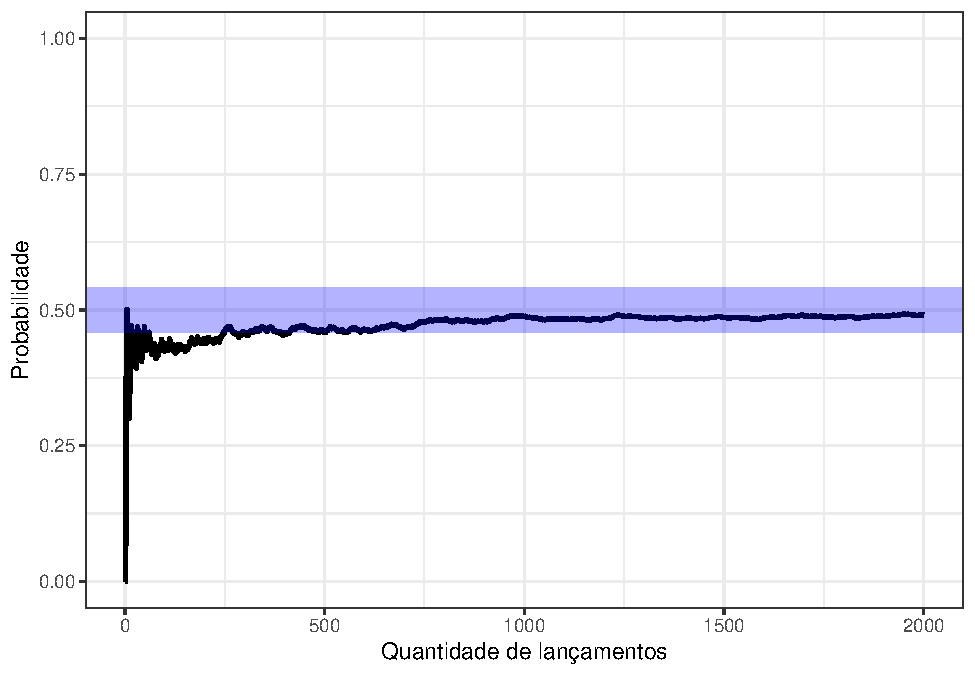
\includegraphics{gitbook-demo_files/figure-latex/unnamed-chunk-11-1.pdf}

Já abaixo, as barras são utilizadas para apresentar as proporções. Um recurso do pacote \texttt{scales} foi utilizado para adequar a visualização das proporções.

\begin{Shaded}
\begin{Highlighting}[]
\KeywordTok{ggplot}\NormalTok{(Dataset, }\KeywordTok{aes}\NormalTok{(}\DataTypeTok{x =}\NormalTok{ country, }\DataTypeTok{y =}\NormalTok{ ..prop.., }\DataTypeTok{group =} \DecValTok{1}\NormalTok{)) }\OperatorTok{+}\StringTok{ }
\StringTok{  }\KeywordTok{geom_bar}\NormalTok{(}\DataTypeTok{stat =} \StringTok{"count"}\NormalTok{) }\OperatorTok{+}
\StringTok{  }\KeywordTok{scale_y_continuous}\NormalTok{(}\DataTypeTok{labels =}\NormalTok{ scales}\OperatorTok{::}\KeywordTok{percent_format}\NormalTok{()) }\OperatorTok{+}
\StringTok{  }\KeywordTok{labs}\NormalTok{(}\DataTypeTok{x =} \StringTok{"País"}\NormalTok{, }\DataTypeTok{title =} \StringTok{"Proporção de participantes em cada país investigado"}\NormalTok{)}
\end{Highlighting}
\end{Shaded}

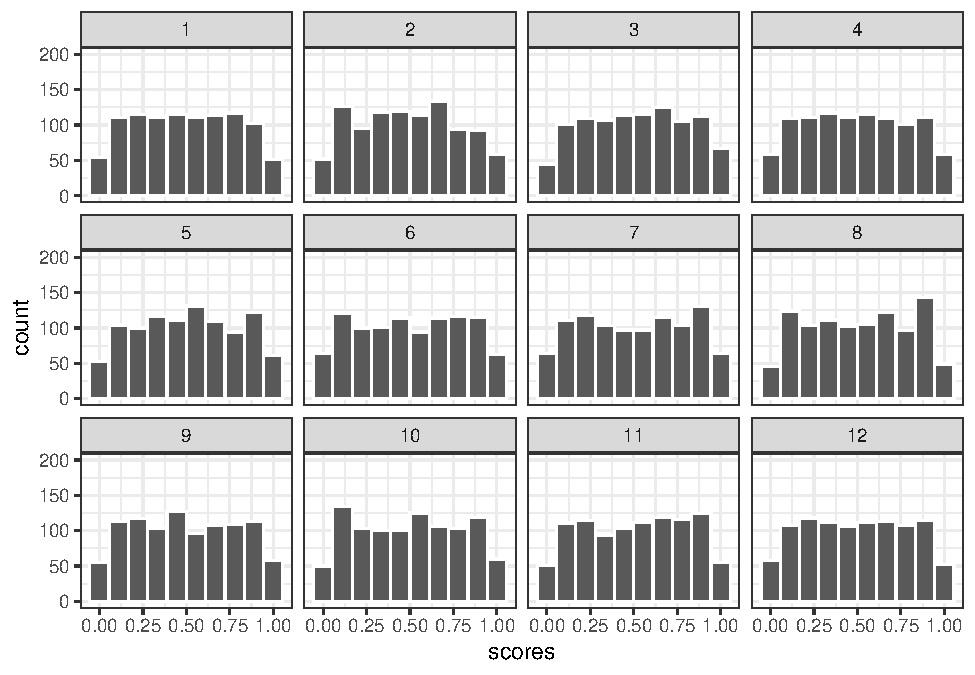
\includegraphics{gitbook-demo_files/figure-latex/unnamed-chunk-12-1.pdf}

É também possível apresentar as proporções em uma única barra, cujas cores variam em função dos grupos.

\begin{Shaded}
\begin{Highlighting}[]
\KeywordTok{ggplot}\NormalTok{(Dataset, }\KeywordTok{aes}\NormalTok{(}\DataTypeTok{x=} \StringTok{""}\NormalTok{, }\DataTypeTok{y =} \StringTok{"perc"}\NormalTok{, }\DataTypeTok{fill =}\NormalTok{ country)) }\OperatorTok{+}
\StringTok{  }\KeywordTok{geom_bar}\NormalTok{(}\DataTypeTok{stat =} \StringTok{"identity"}\NormalTok{, }\DataTypeTok{position =} \StringTok{"stack"}\NormalTok{) }\OperatorTok{+}
\StringTok{  }\KeywordTok{coord_flip}\NormalTok{()}
\end{Highlighting}
\end{Shaded}

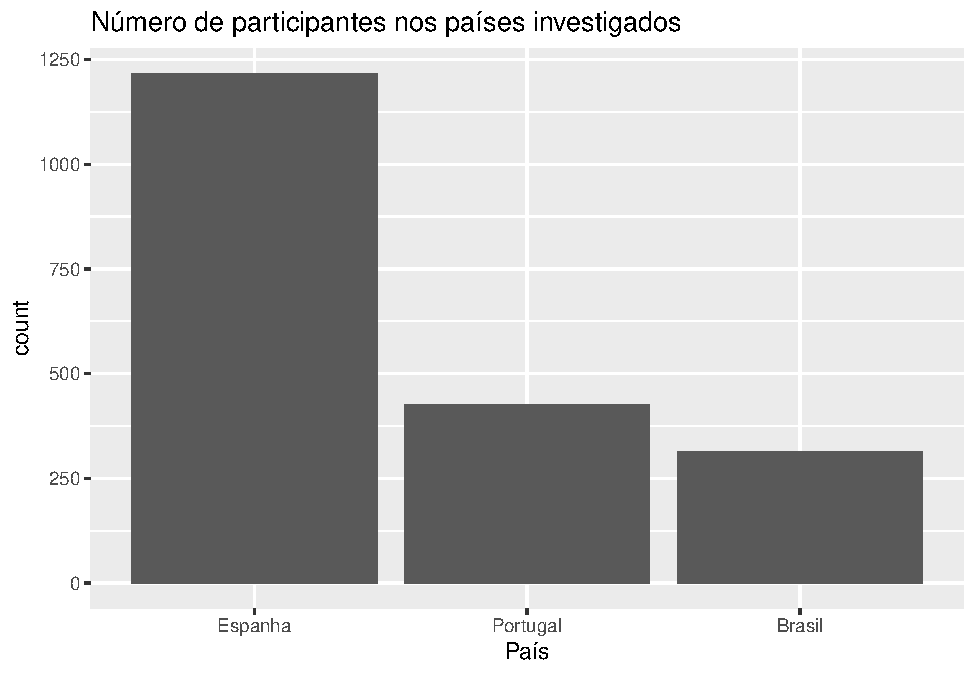
\includegraphics{gitbook-demo_files/figure-latex/unnamed-chunk-13-1.pdf}

Finalmente, o gráfico de setor (as vezes chamado de pizza ou torta) pode também ser utilizado. O aspecto principal desse gráfico é apresentar os setores de maneira proporcional às frequências.

\begin{Shaded}
\begin{Highlighting}[]
\KeywordTok{ggplot}\NormalTok{(Dataset, }\KeywordTok{aes}\NormalTok{(}\DataTypeTok{x=} \StringTok{""}\NormalTok{, }\DataTypeTok{y =} \StringTok{"perc"}\NormalTok{, }\DataTypeTok{fill =}\NormalTok{ country)) }\OperatorTok{+}
\StringTok{  }\KeywordTok{geom_bar}\NormalTok{(}\DataTypeTok{width =} \DecValTok{1}\NormalTok{, }\DataTypeTok{stat =} \StringTok{"identity"}\NormalTok{) }\OperatorTok{+}\StringTok{ }
\StringTok{  }\KeywordTok{coord_polar}\NormalTok{(}\DataTypeTok{theta=}\StringTok{"y"}\NormalTok{) }\OperatorTok{+}
\StringTok{  }\KeywordTok{labs}\NormalTok{(}\DataTypeTok{title =} \StringTok{"Proporção de participantes em cada país"}\NormalTok{)}
\end{Highlighting}
\end{Shaded}

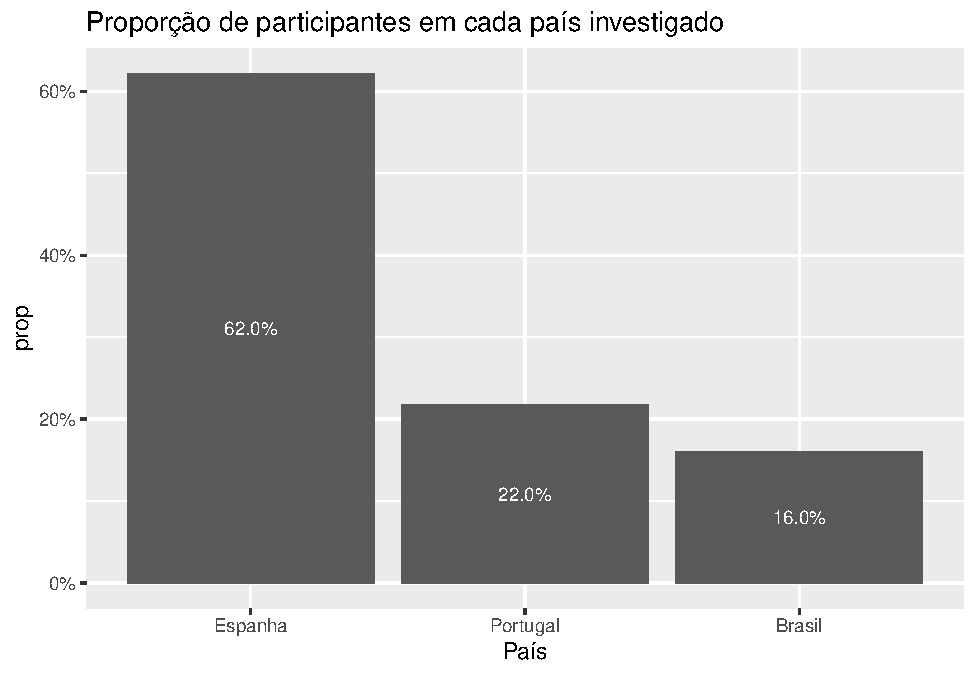
\includegraphics{gitbook-demo_files/figure-latex/unnamed-chunk-14-1.pdf}

\hypertarget{variuxe1vel-contuxednua}{%
\section{1 variável contínua}\label{variuxe1vel-contuxednua}}

Quando uma única variável é apresentada no gráfico e ela é continua, os gráficos adequados são o histograma, densidade e o boxplot.

Abaixo um histograma da idade dos participantes:

\begin{Shaded}
\begin{Highlighting}[]
\KeywordTok{ggplot}\NormalTok{(Dataset, }\KeywordTok{aes}\NormalTok{(}\DataTypeTok{x =}\NormalTok{ age)) }\OperatorTok{+}
\StringTok{  }\KeywordTok{geom_histogram}\NormalTok{(}\DataTypeTok{bins =} \DecValTok{30}\NormalTok{, }\DataTypeTok{color =} \StringTok{"black"}\NormalTok{, }\DataTypeTok{fill =} \StringTok{"lightgrey"}\NormalTok{) }\OperatorTok{+}
\StringTok{  }\KeywordTok{labs}\NormalTok{(}\DataTypeTok{title =} \StringTok{"Distribuição da idade dos participantes"}\NormalTok{)}
\end{Highlighting}
\end{Shaded}

\begin{verbatim}
## Warning: Removed 28 rows containing non-finite values (stat_bin).
\end{verbatim}

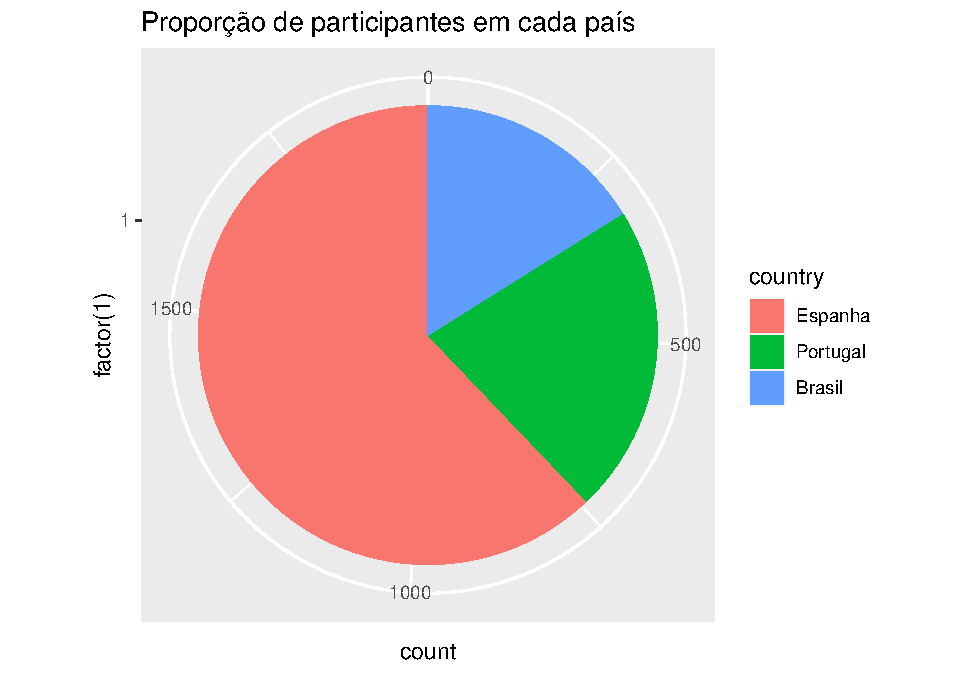
\includegraphics{gitbook-demo_files/figure-latex/unnamed-chunk-15-1.pdf}

Abaixo um gráfico de densidade da idade:

\begin{Shaded}
\begin{Highlighting}[]
\KeywordTok{ggplot}\NormalTok{(Dataset, }\KeywordTok{aes}\NormalTok{(}\DataTypeTok{x =}\NormalTok{ age)) }\OperatorTok{+}
\StringTok{  }\KeywordTok{geom_density}\NormalTok{(}\DataTypeTok{fill =} \StringTok{"lightgray"}\NormalTok{) }\OperatorTok{+}
\StringTok{  }\KeywordTok{labs}\NormalTok{(}\DataTypeTok{title =} \StringTok{"Distribuição da idade dos participantes"}\NormalTok{)}
\end{Highlighting}
\end{Shaded}

\begin{verbatim}
## Warning: Removed 28 rows containing non-finite values (stat_density).
\end{verbatim}

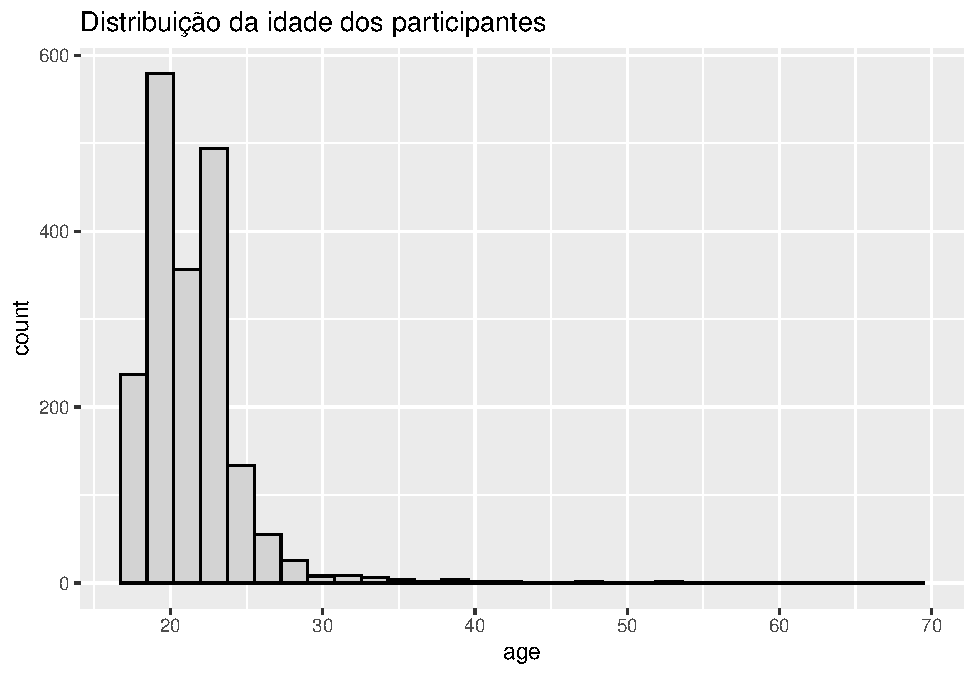
\includegraphics{gitbook-demo_files/figure-latex/unnamed-chunk-16-1.pdf}

Por sua vez, abaixo o boxplot dessa mesma variável:

\begin{Shaded}
\begin{Highlighting}[]
\KeywordTok{ggplot}\NormalTok{(Dataset, }\KeywordTok{aes}\NormalTok{(}\DataTypeTok{y =}\NormalTok{ age, }\DataTypeTok{x =} \StringTok{""}\NormalTok{)) }\OperatorTok{+}
\StringTok{  }\KeywordTok{geom_boxplot}\NormalTok{() }\OperatorTok{+}
\StringTok{  }\KeywordTok{labs}\NormalTok{(}\DataTypeTok{title =} \StringTok{"Distribuição da idade dos participantes"}\NormalTok{)}
\end{Highlighting}
\end{Shaded}

\begin{verbatim}
## Warning: Removed 28 rows containing non-finite values (stat_boxplot).
\end{verbatim}

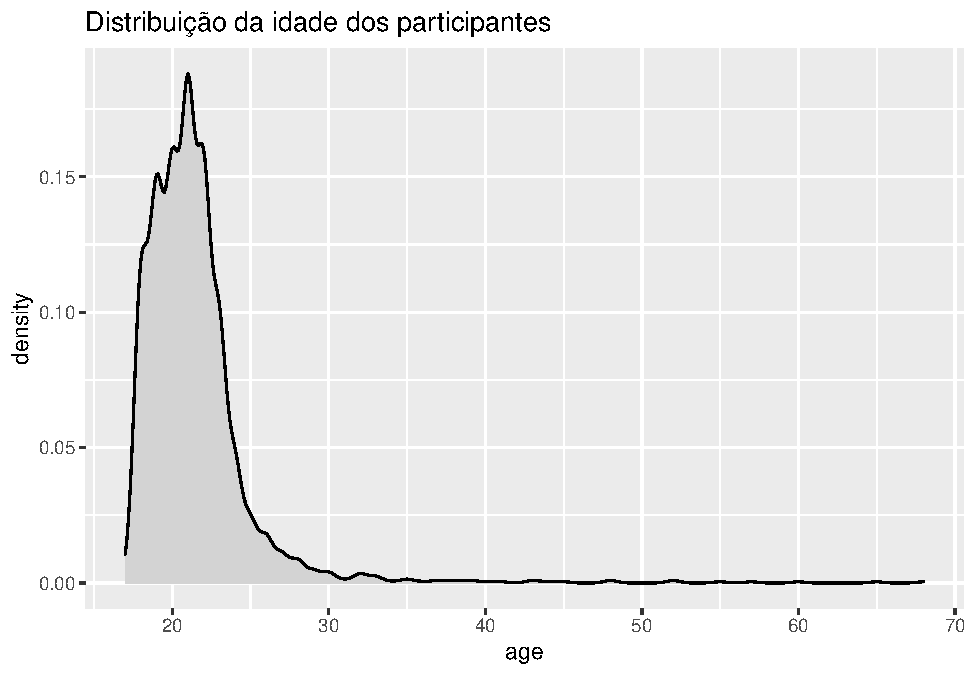
\includegraphics{gitbook-demo_files/figure-latex/unnamed-chunk-17-1.pdf}

O boxplot tem vantagens em comparação com os outros gráficos apresentados até agora. A caixa reúne 50\% da distribuição (Q1, Mediana e Q3) e os bigodes são construídos com base em \texttt{Q1\ -\ 1.5*IQR} e \texttt{Q3\ +\ 1.5*IQR}.

Apesar de algo difícil de visualizar ao início, a informação apresentada no boxplot e no gráfico de densidade são iguais.

\begin{Shaded}
\begin{Highlighting}[]
\NormalTok{a <-}\StringTok{ }\KeywordTok{ggplot}\NormalTok{(Dataset, }\KeywordTok{aes}\NormalTok{(}\DataTypeTok{x =}\NormalTok{ age)) }\OperatorTok{+}
\StringTok{  }\KeywordTok{geom_density}\NormalTok{(}\DataTypeTok{fill =} \StringTok{"lightgray"}\NormalTok{)}

\NormalTok{b <-}\StringTok{ }\KeywordTok{ggplot}\NormalTok{(Dataset, }\KeywordTok{aes}\NormalTok{(}\DataTypeTok{y =}\NormalTok{ age, }\DataTypeTok{x =} \StringTok{""}\NormalTok{)) }\OperatorTok{+}
\StringTok{  }\KeywordTok{geom_boxplot}\NormalTok{() }\OperatorTok{+}
\StringTok{  }\KeywordTok{coord_flip}\NormalTok{()}

\KeywordTok{grid.arrange}\NormalTok{(a,b, }\DataTypeTok{top =} \StringTok{"Distribuição da idade dos participantes"}\NormalTok{)}
\end{Highlighting}
\end{Shaded}

\begin{verbatim}
## Warning: Removed 28 rows containing non-finite values (stat_density).
\end{verbatim}

\begin{verbatim}
## Warning: Removed 28 rows containing non-finite values (stat_boxplot).
\end{verbatim}

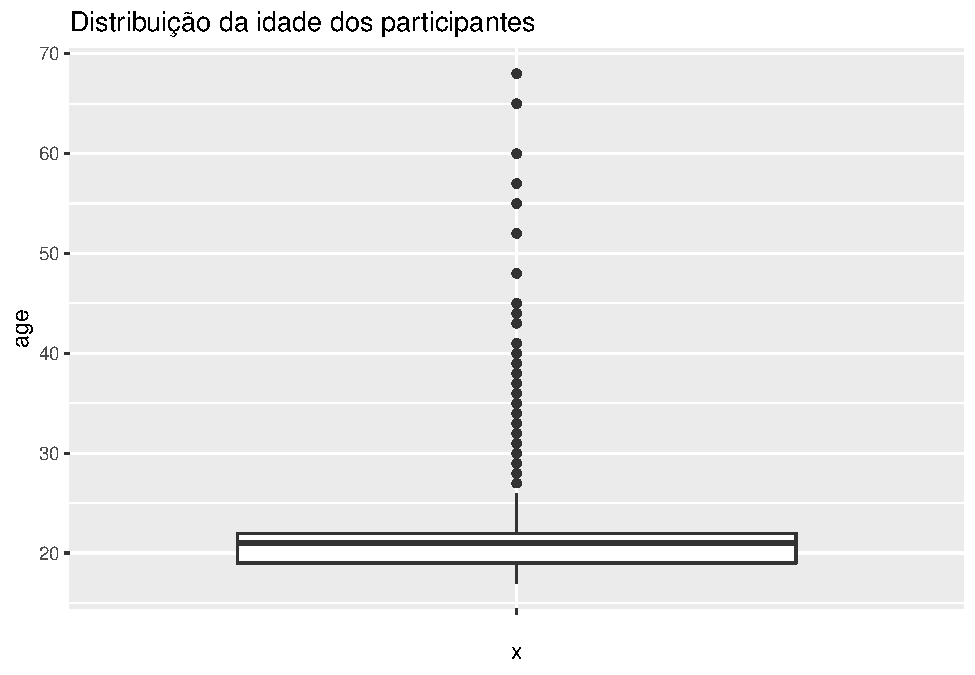
\includegraphics{gitbook-demo_files/figure-latex/unnamed-chunk-18-1.pdf}

\hypertarget{variuxe1veis-vi-discreta}{%
\section{2 variáveis (VI discreta)}\label{variuxe1veis-vi-discreta}}

Por definição, os gráficos de barras ou colunas (considerando aqui as barras de erro) e o boxplot são adequados para apresentar essa relação. Basicamente, esses gráficos permitem verificar a \textbf{diferença} entre os grupos.

O gráfico abaixo mostra os resultados do Inventário Beck de Ansiedade entre 3 países investigados. As barras de erro são importantes para verificar, inicialmente, as possíveis diferenças significativas entre os países.

\begin{Shaded}
\begin{Highlighting}[]
\KeywordTok{ggplot}\NormalTok{(Dataset, }\KeywordTok{aes}\NormalTok{(}\DataTypeTok{x =}\NormalTok{ country, }\DataTypeTok{y =}\NormalTok{ bai_sum)) }\OperatorTok{+}
\StringTok{  }\KeywordTok{geom_bar}\NormalTok{(}\DataTypeTok{stat =} \StringTok{"summary"}\NormalTok{) }\OperatorTok{+}
\StringTok{  }\KeywordTok{stat_summary}\NormalTok{(}\DataTypeTok{geom =} \StringTok{"errorbar"}\NormalTok{,}\DataTypeTok{fun.data =}\NormalTok{ mean_se) }\OperatorTok{+}
\StringTok{  }\KeywordTok{labs}\NormalTok{(}\DataTypeTok{title =} \StringTok{"Resultados da escala de ansiedade em função do país investigado"}\NormalTok{)}
\end{Highlighting}
\end{Shaded}

\begin{verbatim}
## No summary function supplied, defaulting to `mean_se()
\end{verbatim}

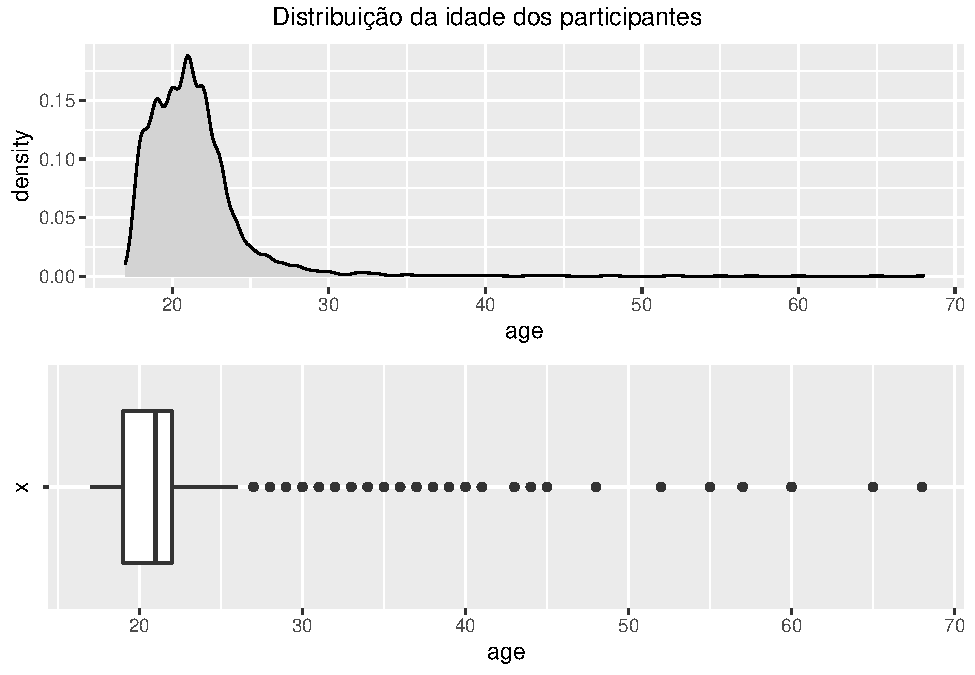
\includegraphics{gitbook-demo_files/figure-latex/unnamed-chunk-19-1.pdf}

O boxplot a seguir também é um gráfico indicado:

\begin{Shaded}
\begin{Highlighting}[]
\KeywordTok{ggplot}\NormalTok{(Dataset, }\KeywordTok{aes}\NormalTok{(}\DataTypeTok{x =}\NormalTok{ country, }\DataTypeTok{y =}\NormalTok{ bai_sum)) }\OperatorTok{+}
\StringTok{  }\KeywordTok{geom_boxplot}\NormalTok{()}
\end{Highlighting}
\end{Shaded}

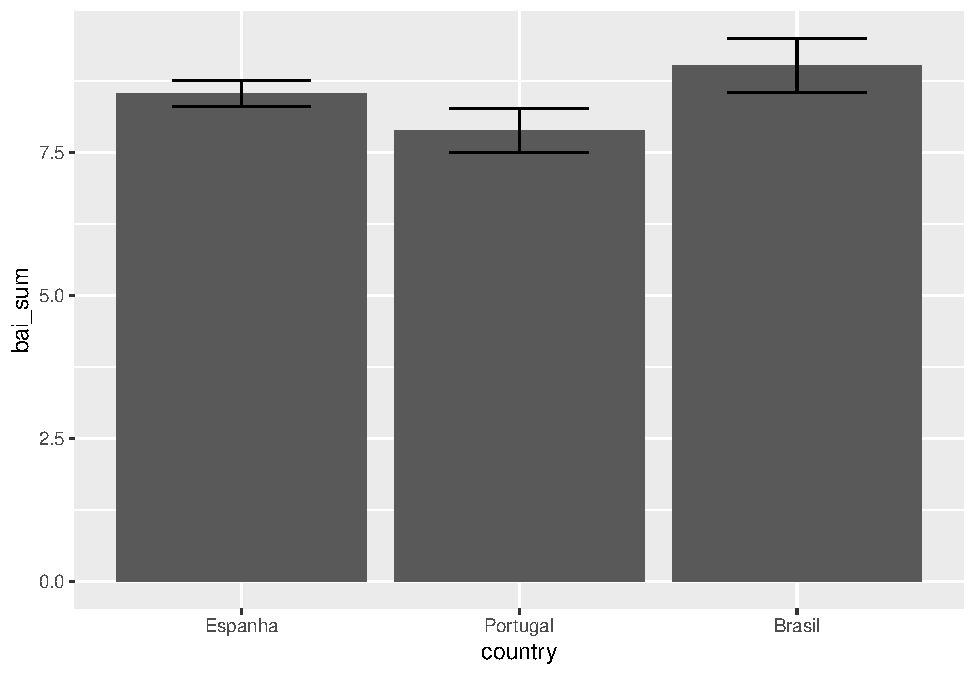
\includegraphics{gitbook-demo_files/figure-latex/unnamed-chunk-20-1.pdf}

\hypertarget{variuxe1veis-vi-contuxednua}{%
\section{2 variáveis (VI contínua)}\label{variuxe1veis-vi-contuxednua}}

Assumindo que a VI é contínua e a VD também, o gráfico de pontos e de dispersão são virtualmente identicos e indicados. Esses gráficos permitem verificar a \textbf{associação} entre as variáveis. No ggoplot, o argumento \texttt{geom\_point} e \texttt{geom\_jitter} são possíveis. Abaixo, utilizando os pontos.

\begin{Shaded}
\begin{Highlighting}[]
\KeywordTok{ggplot}\NormalTok{(Dataset, }\KeywordTok{aes}\NormalTok{(}\DataTypeTok{x =}\NormalTok{ age, }\DataTypeTok{y =}\NormalTok{ bai_sum)) }\OperatorTok{+}
\StringTok{  }\KeywordTok{geom_point}\NormalTok{() }\OperatorTok{+}
\StringTok{  }\KeywordTok{labs}\NormalTok{(}\DataTypeTok{title =} \StringTok{"Resultados da escala de ansiedade em função da idade do participante"}\NormalTok{)}
\end{Highlighting}
\end{Shaded}

\begin{verbatim}
## Warning: Removed 28 rows containing missing values (geom_point).
\end{verbatim}

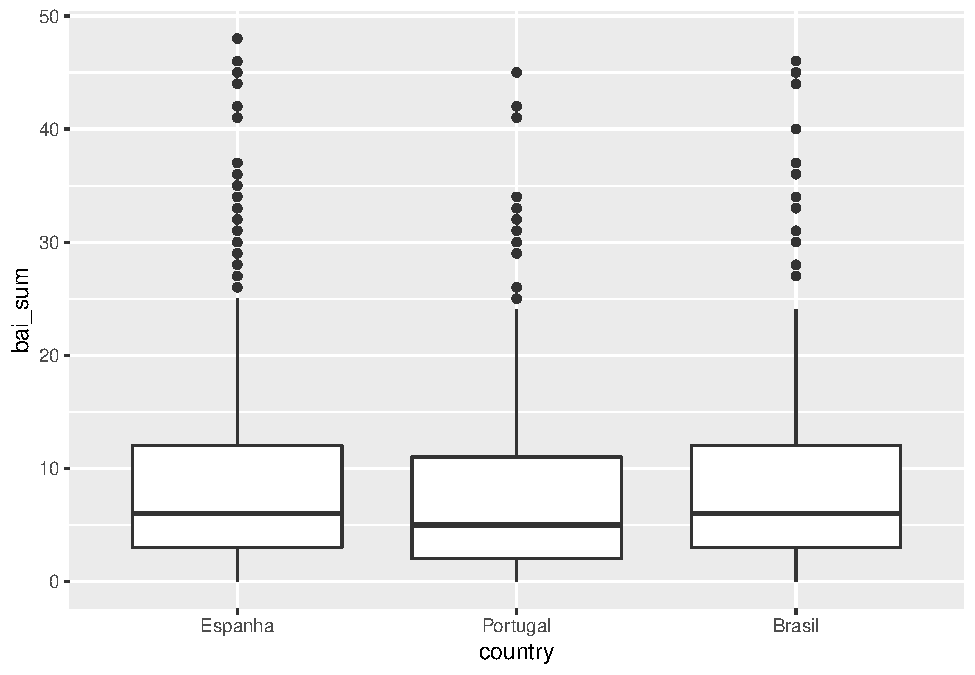
\includegraphics{gitbook-demo_files/figure-latex/unnamed-chunk-21-1.pdf}

Abaixo, utilizando o jitter

\begin{Shaded}
\begin{Highlighting}[]
\KeywordTok{ggplot}\NormalTok{(Dataset, }\KeywordTok{aes}\NormalTok{(}\DataTypeTok{x =}\NormalTok{ age, }\DataTypeTok{y =}\NormalTok{ bai_sum)) }\OperatorTok{+}
\StringTok{  }\KeywordTok{geom_jitter}\NormalTok{() }\OperatorTok{+}
\StringTok{  }\KeywordTok{labs}\NormalTok{(}\DataTypeTok{title =} \StringTok{"Resultados da escala de ansiedade em função da idade do participante"}\NormalTok{)}
\end{Highlighting}
\end{Shaded}

\begin{verbatim}
## Warning: Removed 28 rows containing missing values (geom_point).
\end{verbatim}

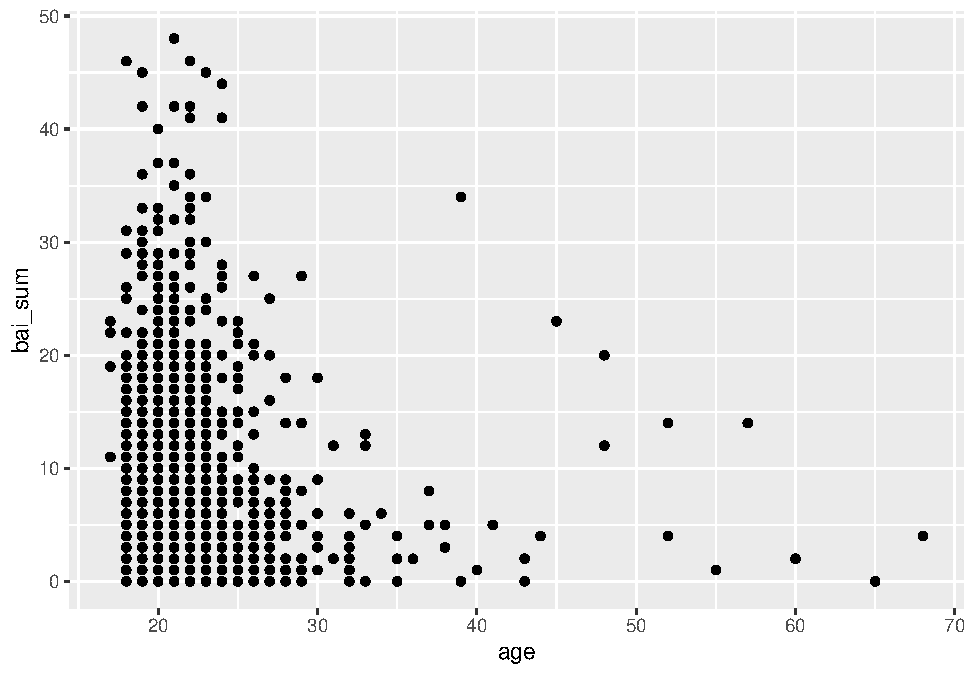
\includegraphics{gitbook-demo_files/figure-latex/unnamed-chunk-22-1.pdf}

Tradicionalmente, de maneira análoga às barras de erros apresentadas em gráficos cujas VIs são discretas, adiciona-se uma linha de regressão amostral quando a VI é contínua, tal como apresentado a seguir.

\begin{Shaded}
\begin{Highlighting}[]
\KeywordTok{ggplot}\NormalTok{(Dataset, }\KeywordTok{aes}\NormalTok{(}\DataTypeTok{x =}\NormalTok{ age, }\DataTypeTok{y =}\NormalTok{ bai_sum)) }\OperatorTok{+}
\StringTok{  }\KeywordTok{geom_jitter}\NormalTok{() }\OperatorTok{+}
\StringTok{  }\KeywordTok{geom_smooth}\NormalTok{(}\DataTypeTok{method =} \StringTok{"lm"}\NormalTok{) }\OperatorTok{+}
\StringTok{  }\KeywordTok{labs}\NormalTok{(}\DataTypeTok{title =} \StringTok{"Resultados da escala de ansiedade em função da idade do participante"}\NormalTok{)}
\end{Highlighting}
\end{Shaded}

\begin{verbatim}
## Warning: Removed 28 rows containing non-finite values (stat_smooth).
\end{verbatim}

\begin{verbatim}
## Warning: Removed 28 rows containing missing values (geom_point).
\end{verbatim}

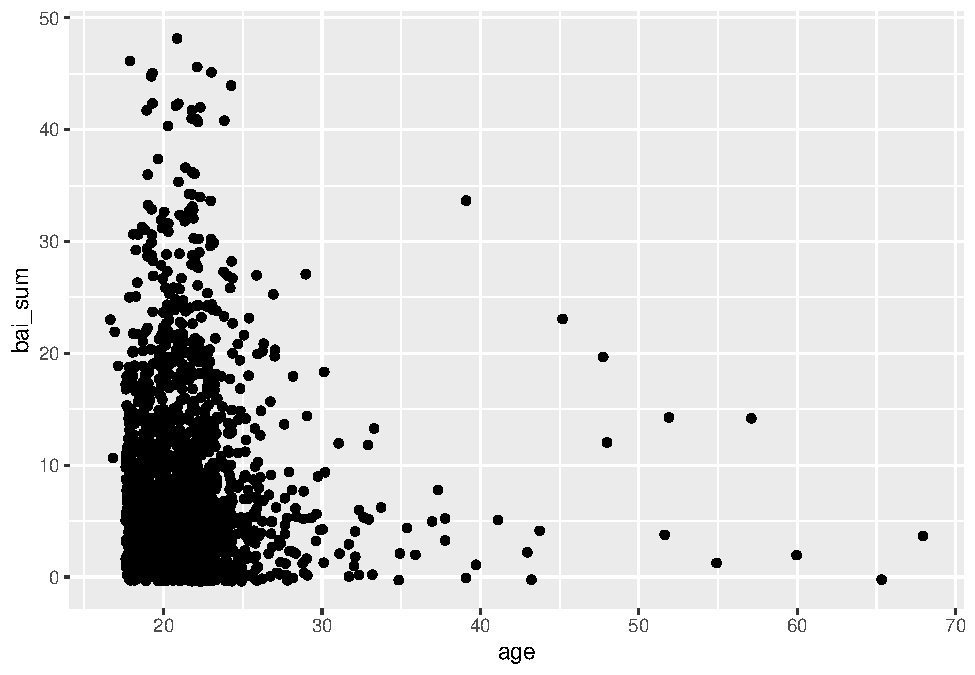
\includegraphics{gitbook-demo_files/figure-latex/unnamed-chunk-23-1.pdf}

\hypertarget{outros-gruxe1ficos}{%
\section{Outros gráficos}\label{outros-gruxe1ficos}}

Evidentemente, é possível apresentar mais informações nos gráficos com mais de um variável apresentada, desde que elas sejam relacionadas ao problema de pesquisa estudado e não sobrecarreguem a visualização dos resultados. Frequentemente, as informações adicionais são feitas pela inclusão de \textbf{clusters} ou \textbf{agrupamentos}. Isso é tanto possível em gráficos cuja VI seja discreta quanto contínua.

No exemplo abaixo, o gráfico dos resultados do Inventário Beck de Ansiedade entre os 3 países investigados (VI discreta) agora está agrupado pelo sexo do participante.

\begin{Shaded}
\begin{Highlighting}[]
\NormalTok{Dataset }\OperatorTok\StringTok{ }
\StringTok{  }\KeywordTok{filter}\NormalTok{(}\OperatorTok{!}\KeywordTok{is.na}\NormalTok{(sex)) }\OperatorTok\StringTok{ }
\StringTok{  }\KeywordTok{ggplot}\NormalTok{(., }\KeywordTok{aes}\NormalTok{(}\DataTypeTok{x =}\NormalTok{ country, }\DataTypeTok{y =}\NormalTok{ bai_sum, }\DataTypeTok{fill =}\NormalTok{ sex)) }\OperatorTok{+}
\StringTok{  }\KeywordTok{geom_bar}\NormalTok{(}\DataTypeTok{stat =} \StringTok{"summary"}\NormalTok{, }\DataTypeTok{position =} \StringTok{"dodge"}\NormalTok{) }\OperatorTok{+}
\StringTok{  }\KeywordTok{stat_summary}\NormalTok{(}\DataTypeTok{geom=}\StringTok{"errorbar"}\NormalTok{, }\DataTypeTok{fun.data =}\NormalTok{ mean_se, }\DataTypeTok{position =} \KeywordTok{position_dodge}\NormalTok{(}\FloatTok{0.95}\NormalTok{)) }\OperatorTok{+}
\StringTok{  }\KeywordTok{labs}\NormalTok{(}\DataTypeTok{title =} \StringTok{"Resultados da escala de ansiedade em função da idade e sexo do participante"}\NormalTok{)}
\end{Highlighting}
\end{Shaded}

\begin{verbatim}
## No summary function supplied, defaulting to `mean_se()
\end{verbatim}

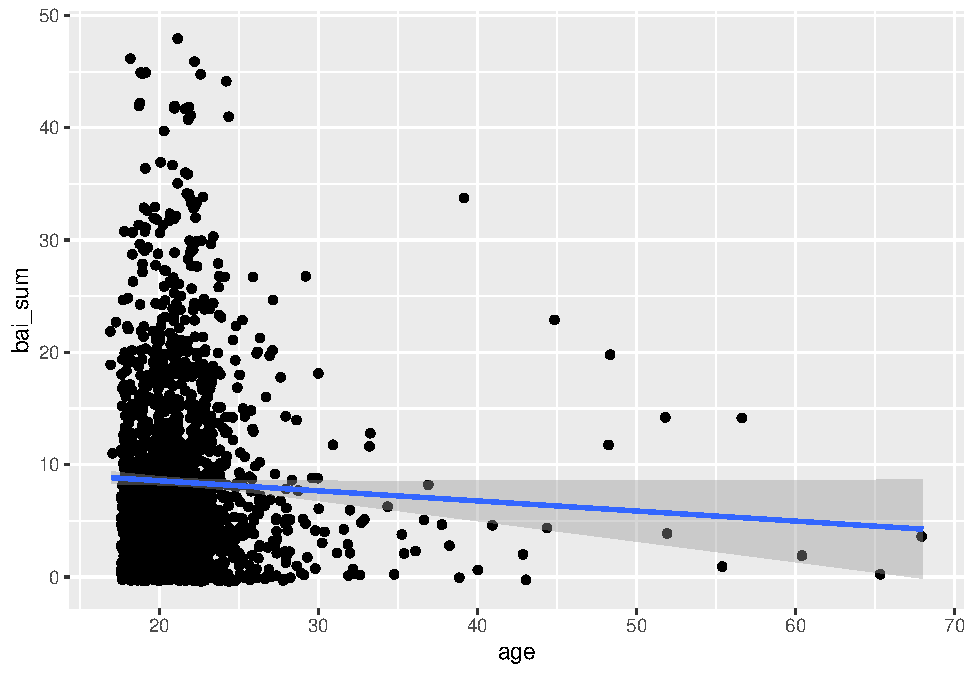
\includegraphics{gitbook-demo_files/figure-latex/unnamed-chunk-24-1.pdf}

Já no exemplo abaixo, a relação entre idade e pontuação no Inventário Beck de Ansiedade está agora agrupada pelo sexo do participante.

\begin{Shaded}
\begin{Highlighting}[]
\NormalTok{Dataset }\OperatorTok\StringTok{ }
\StringTok{  }\KeywordTok{filter}\NormalTok{(}\OperatorTok{!}\KeywordTok{is.na}\NormalTok{(sex)) }\OperatorTok\StringTok{ }
\StringTok{  }\KeywordTok{ggplot}\NormalTok{(., }\KeywordTok{aes}\NormalTok{(}\DataTypeTok{x =}\NormalTok{ age, }\DataTypeTok{y =}\NormalTok{ bai_sum, }\DataTypeTok{color =}\NormalTok{ sex)) }\OperatorTok{+}
\StringTok{  }\KeywordTok{geom_jitter}\NormalTok{() }\OperatorTok{+}
\StringTok{  }\KeywordTok{geom_smooth}\NormalTok{(}\DataTypeTok{method =} \StringTok{"lm"}\NormalTok{) }\OperatorTok{+}
\StringTok{  }\KeywordTok{labs}\NormalTok{(}\DataTypeTok{title =} \StringTok{"Resultados da escala de ansiedade em função da idade e sexo do participante"}\NormalTok{)}
\end{Highlighting}
\end{Shaded}

\begin{verbatim}
## Warning: Removed 24 rows containing non-finite values (stat_smooth).
\end{verbatim}

\begin{verbatim}
## Warning: Removed 24 rows containing missing values (geom_point).
\end{verbatim}

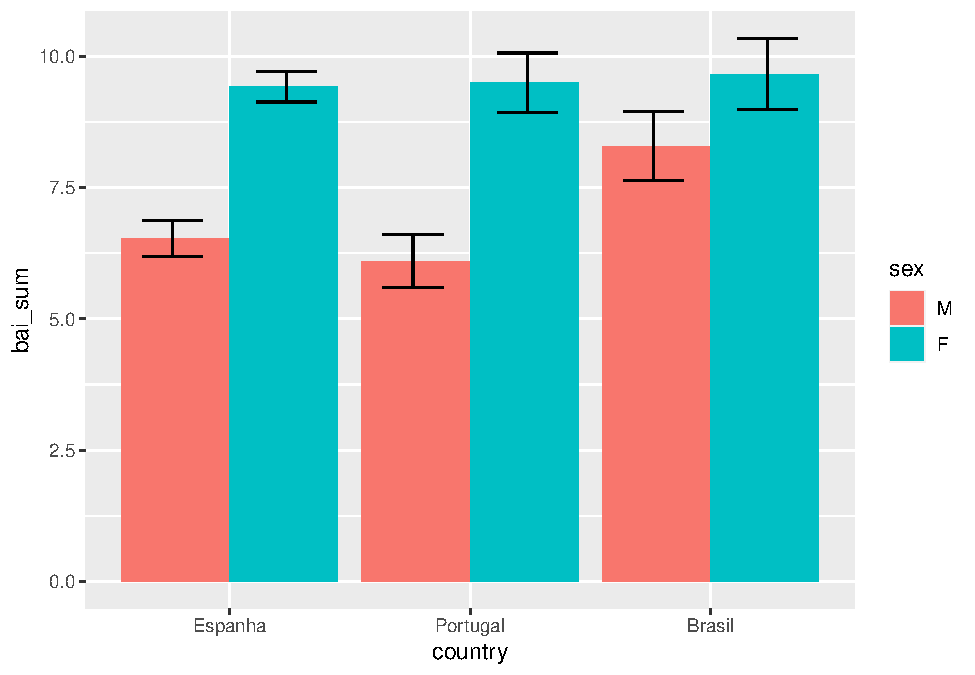
\includegraphics{gitbook-demo_files/figure-latex/unnamed-chunk-25-1.pdf}

Em situações onde existe uma grande quantidade de informação para ser apresentada, os resultados começam a se tornar difíceis de serem entendidos. O gráfico abaixo, por exemplo, é excessivamente carregado de informação e, consequentemente, inadequado.

\begin{Shaded}
\begin{Highlighting}[]
\NormalTok{Dataset }\OperatorTok\StringTok{ }
\StringTok{  }\KeywordTok{filter}\NormalTok{(}\OperatorTok{!}\KeywordTok{is.na}\NormalTok{(sex)) }\OperatorTok\StringTok{ }
\StringTok{  }\KeywordTok{ggplot}\NormalTok{(., }\KeywordTok{aes}\NormalTok{(}\DataTypeTok{x =}\NormalTok{ age, }\DataTypeTok{y =}\NormalTok{ bai_sum, }\DataTypeTok{color =}\NormalTok{ sex, }\DataTypeTok{shape =}\NormalTok{ country)) }\OperatorTok{+}
\StringTok{  }\KeywordTok{geom_jitter}\NormalTok{() }\OperatorTok{+}
\StringTok{  }\KeywordTok{geom_smooth}\NormalTok{(}\DataTypeTok{method =} \StringTok{"lm"}\NormalTok{) }\OperatorTok{+}
\StringTok{  }\KeywordTok{labs}\NormalTok{(}\DataTypeTok{title =} \StringTok{"Resultados da escala de ansiedade em função da idade, país e sexo do participante"}\NormalTok{)}
\end{Highlighting}
\end{Shaded}

\begin{verbatim}
## Warning: Removed 24 rows containing non-finite values (stat_smooth).
\end{verbatim}

\begin{verbatim}
## Warning: Removed 24 rows containing missing values (geom_point).
\end{verbatim}

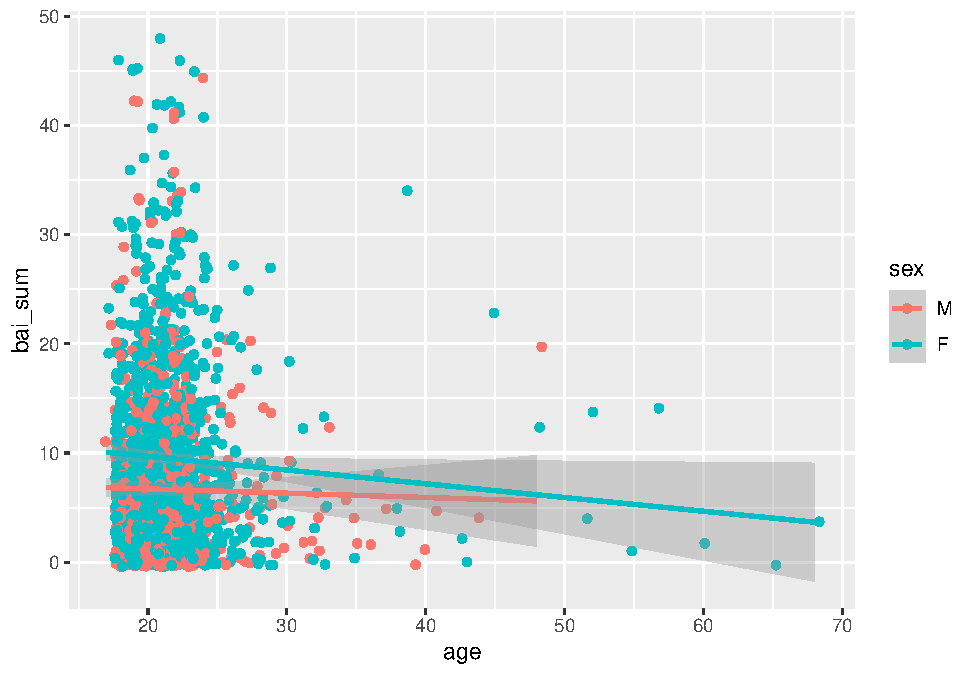
\includegraphics{gitbook-demo_files/figure-latex/unnamed-chunk-26-1.pdf}

Em outro sentido, o gráfico a seguir quebra a apresentação dos resultados por país e, com isso, potencializa que a informação seja melhor compreendida.

\begin{Shaded}
\begin{Highlighting}[]
\NormalTok{Dataset }\OperatorTok\StringTok{ }
\StringTok{  }\KeywordTok{filter}\NormalTok{(}\OperatorTok{!}\KeywordTok{is.na}\NormalTok{(sex)) }\OperatorTok\StringTok{ }
\StringTok{  }\KeywordTok{ggplot}\NormalTok{(., }\KeywordTok{aes}\NormalTok{(}\DataTypeTok{x =}\NormalTok{ age, }\DataTypeTok{y =}\NormalTok{ bai_sum, }\DataTypeTok{color =}\NormalTok{ sex)) }\OperatorTok{+}
\StringTok{  }\KeywordTok{geom_jitter}\NormalTok{() }\OperatorTok{+}
\StringTok{  }\KeywordTok{geom_smooth}\NormalTok{(}\DataTypeTok{method =} \StringTok{"lm"}\NormalTok{) }\OperatorTok{+}
\StringTok{  }\KeywordTok{facet_wrap}\NormalTok{( }\OperatorTok{~}\StringTok{ }\NormalTok{country) }\OperatorTok{+}
\StringTok{  }\KeywordTok{labs}\NormalTok{(}\DataTypeTok{title =} \StringTok{"Resultados da escala de ansiedade em função da idade, país e sexo do participante"}\NormalTok{)}
\end{Highlighting}
\end{Shaded}

\begin{verbatim}
## Warning: Removed 24 rows containing non-finite values (stat_smooth).
\end{verbatim}

\begin{verbatim}
## Warning: Removed 24 rows containing missing values (geom_point).
\end{verbatim}

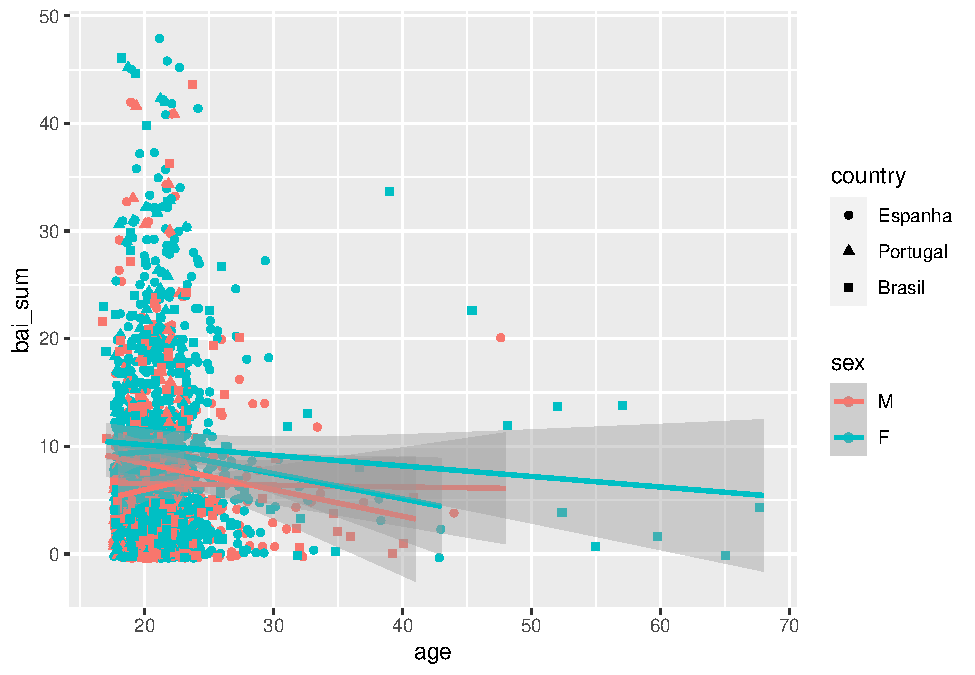
\includegraphics{gitbook-demo_files/figure-latex/unnamed-chunk-27-1.pdf}

\hypertarget{getgitbook}{%
\chapter{Get your GitBook}\label{getgitbook}}

To get your GitBook, you should follow these steps:

\begin{enumerate}
\def\labelenumi{\arabic{enumi}.}
\tightlist
\item
  Go to \url{https://github.com/cjvanlissa/gitbook-demo}
\item
  In the top right of the page, click \texttt{Fork}.\\
  This will copy my \texttt{gitbook-demo} repository to your GitHub account.\\
  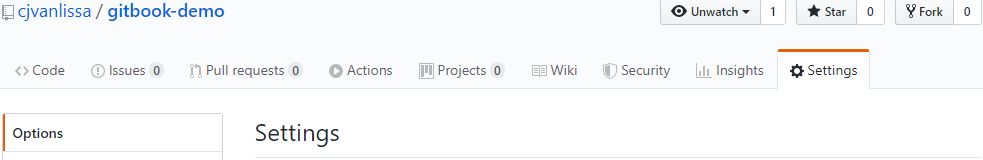
\includegraphics{./img/settings.png}
\item
  My repository is now copied to your account. It is a template repository, which means that you can create a \emph{new repository} based on this one.
\item
  Create a new repository for your own GitBook. Create one for a course you've been wanting to update. In the top-right corner of the GitHub website, click the + icon, and select ``New repository'':\\
  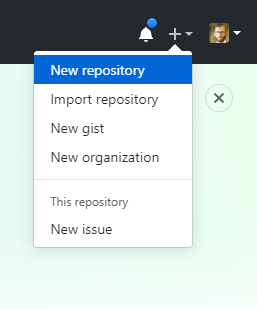
\includegraphics{./img/new_repo.png}
\item
  In the dialog, select the \texttt{gitbook-demo} as ``Repository template'', and give the repository an appropriate name for your course. Then, press \texttt{Create\ repository}:\\
  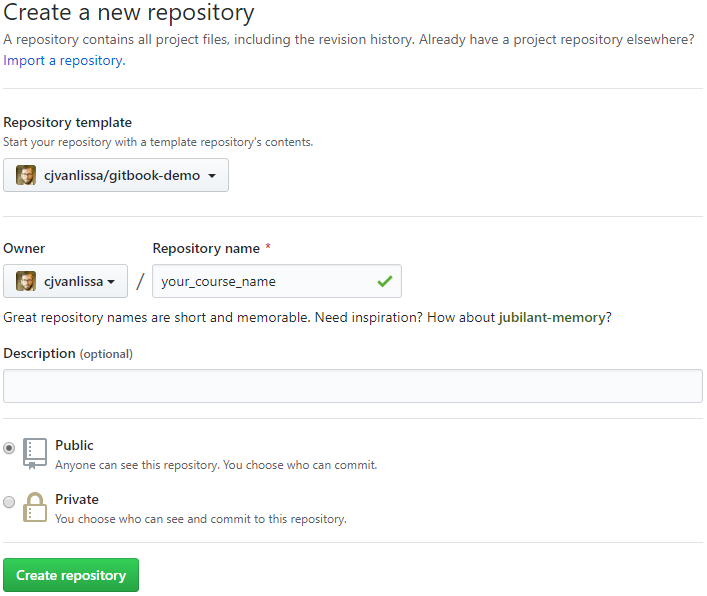
\includegraphics{./img/from_template.png}
\item
  Now, go back to Rstudio on your computer. In Rstudio, click \texttt{File\ \textgreater{}\ New\ Project}. A dialog will open. If you set up Rstudio with Git correctly, the dialog should have an option to create a new project from Version control. Click it:\\
  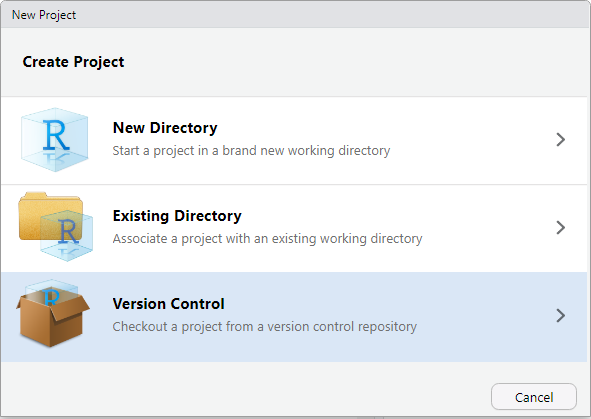
\includegraphics{./img/new_project.png}
\item
  In the next dialog window, you should copy the URL of the GitHub repository you created in \emph{Step 5}, like so:\\
  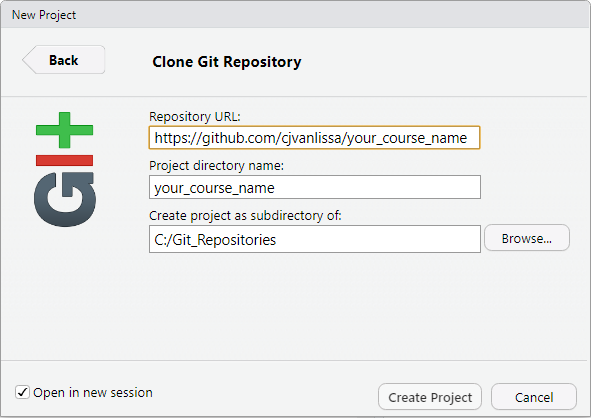
\includegraphics{./img/new_git_project.png}
\item
  Now, in Rstudio, you can open files for editing and create new files (explained in the next Chapter). Open files by clicking them in the Files editor (usually in the bottom right of Rstudio):\\
  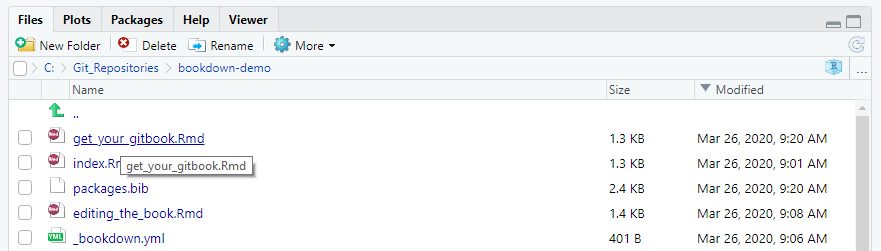
\includegraphics{./img/files_editor.png}
\item
  After you make a change, it will show up in the Git tab (usually in the top right of Rstudio). You must Commit the change locally, and then Push the change to GitHub to update your repo. To Commit, select the file and click the Commit button. Write a short message to describe the changes you made, then click the Commit button again. Now, press Push to send your commits to GitHub.\\
  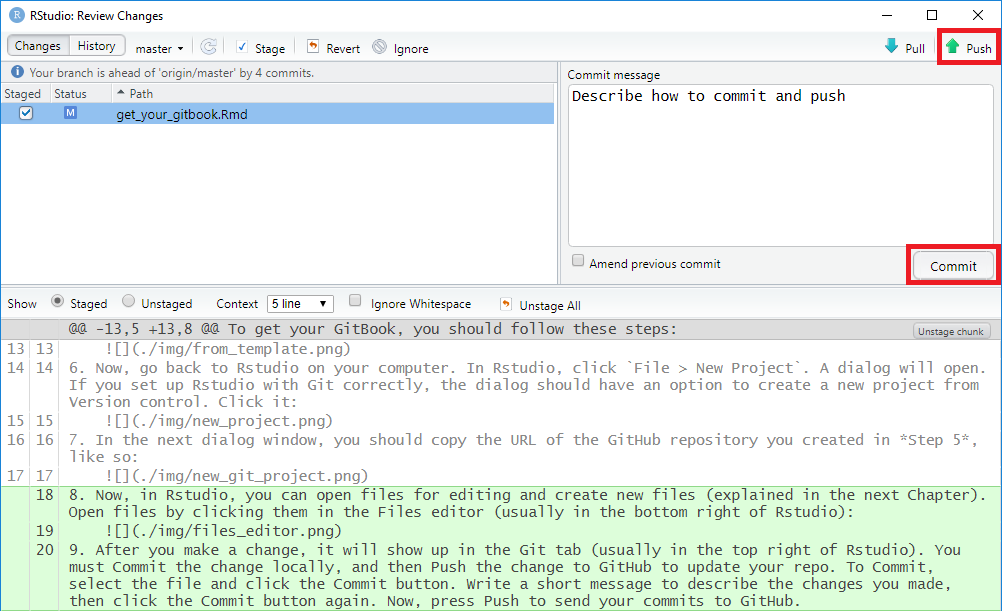
\includegraphics{./img/commit_push.png}
\item
  To render your book as a GitBook, you must ``Build'' it. In the top-right panel of Rstudio, you see a ``Build'' tab. In this tab, simply click the ``Build Book'' button to build your book. You should see a lot of rendering messages, until a window pops up with your brand new GitBook. If you get errors at this stage, you probably made a mistake in preparing your system (see the previous Chapter).\\
  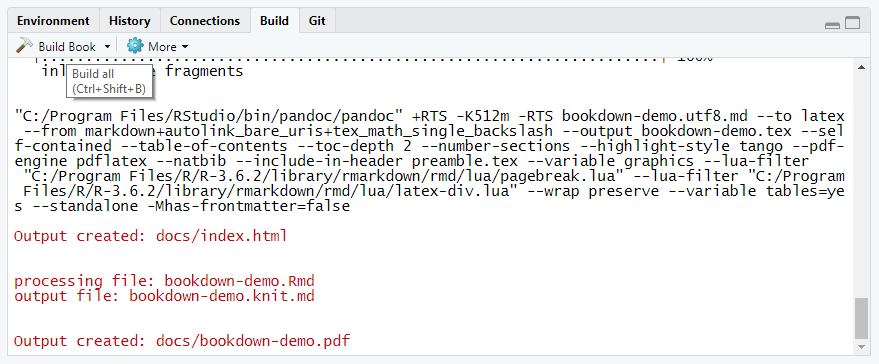
\includegraphics{./img/build_book.png}
\item
  Building the book generated a lot of new files in the \texttt{./docs} directory. This directory contains the website files for your GitBook. Open the Git tab again, verify that the \texttt{./docs} directory is listed, and Commit and Push all of these new files as described in \emph{Step 9}.
\item
  There is only one last remaining task: To publish your GitBook on GitHub pages. Once you do this, any change to the \texttt{./docs} folder that you push to GitHub will lead to an immediate update of your GitBook website. Go back to the GitHub page for your Repository. Click on the \texttt{Settings} tab on the top right of the page:\\
  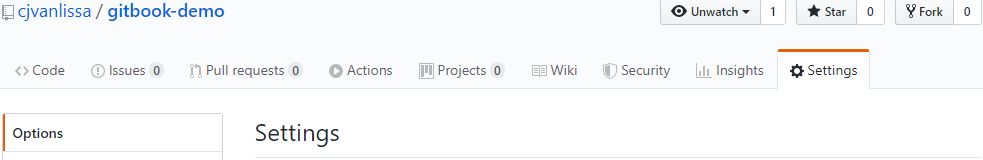
\includegraphics{./img/settings.png}
\item
  On the Settings page, scroll all the way down until you reach a section called \texttt{GitHub\ Pages}. There, under the ``Source'' heading, click the word \texttt{None}, and select \texttt{master\ branch\ /docs\ folder}. When you select it, the page will update, and if you scroll back down to the \texttt{GitHub\ Pages} section, you will see the URL where your GitBook is published. The first time, it will take a few minutes for your GitBook to come online. When you publish updates to the GitBook however (simply by following \emph{Step 11} again), the update will be near-instantaneous. The Pages section should now look like this (and that is hopefully the link where you found this book):\\
  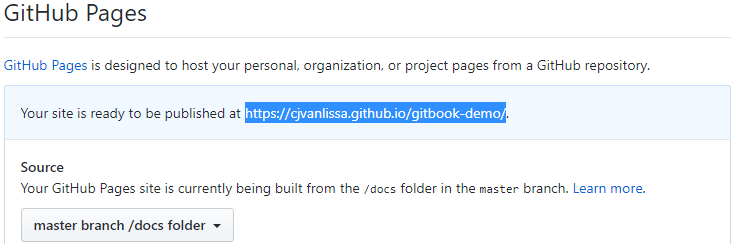
\includegraphics{./img/pages_published.png}
\end{enumerate}

\hypertarget{editing-the-book}{%
\chapter{Editing the book}\label{editing-the-book}}

The contents of the book are written in \textbf{RMarkdown}. You can use any formatting code that Pandoc's Markdown supports, e.g., a math equation \(a^2 + b^2 = c^2\). Moreover, you can include chunks of R-code, like this:

The results of these chunks can be rendered to the GitBook:

\begin{verbatim}
## [1] "This is an R-command!"
\end{verbatim}

To edit the book, you can change the text in the \texttt{.Rmd} files. Each Rmd file should contain \textbf{one and only one} chapter. A chapter is defined by the first-level heading \texttt{\#}, e.g., \texttt{\#\ Editing\ the\ book}.

Any sub-headings within the chapter are indicated with several \texttt{\#} signs, e.g., \texttt{\#\#} (level 2) and \texttt{\#\#\#} (level 3).

\hypertarget{creating-new-chapters}{%
\section{Creating new chapters}\label{creating-new-chapters}}

To create a new chapter, you must follow two steps: 1) Create the file, and 2) Include it in the list of chapters.

First, to create the file for a new chapter in Rstudio, click \texttt{File\ \textgreater{}\ New\ File\ \textgreater{}\ Text\ file}. At the top of the file, write your chapter heading, as explained above. Then, click \texttt{File\ \textgreater{}\ Save}. Save the file as \texttt{.Rmd}, without spaces in the file name, e.g.: \texttt{editing\_the\_book.Rmd}.

Second, to include it in the list of chapters, open the file \texttt{\_bookdown.yml} (click it in the Files explorer in the bottom right of Rstudio). This file has a list of \texttt{.Rmd} files to be included in the book. In this example, the list looks like this:

\begin{Shaded}
\begin{Highlighting}[]
\NormalTok{tmp <-}\StringTok{ }\KeywordTok{readLines}\NormalTok{(}\StringTok{"_bookdown.yml"}\NormalTok{)}
\KeywordTok{cat}\NormalTok{(tmp[}\KeywordTok{grep}\NormalTok{(}\StringTok{"^rmd_files"}\NormalTok{, tmp)}\OperatorTok{:}\KeywordTok{grep}\NormalTok{(}\StringTok{"references}\CharTok{\textbackslash{}\textbackslash{}}\StringTok{.Rmd"}\NormalTok{, tmp)], }\DataTypeTok{sep =} \StringTok{"}\CharTok{\textbackslash{}n}\StringTok{"}\NormalTok{)}
\end{Highlighting}
\end{Shaded}

rmd\_files: {[}``index.Rmd'',
``prerequisites.Rmd'',
``get\_your\_gitbook.Rmd'',
``editing\_the\_book.Rmd'',
``figures\_tables.Rmd'',
``examples.Rmd'',
``open\_educational.Rmd'',
``licenses.Rmd'',
``references.Rmd''{]}

Insert the file name of your new chapter in the desired position in this list.

\hypertarget{linking-across-chapters}{%
\section{Linking across chapters}\label{linking-across-chapters}}

You can label chapter and section titles using \texttt{\{\#label\}} after them. The labels can be used as cross-references. For example, we can link to Chapter \ref{figtab}. If you do not manually label chapters, there will be automatic labels anyway, e.g., Chapter \ref{examples}.

\hypertarget{advanced-editing}{%
\section{Advanced editing}\label{advanced-editing}}

The convenient \href{https://rstudio.com/wp-content/uploads/2016/03/rmarkdown-cheatsheet-2.0.pdf}{Rmarkdown Cheat Sheet} by Rstudio covers most of the knowledge required for advanced Rmarkdown editing. You can print it out and stick it to your wall!

\hypertarget{figtab}{%
\chapter{Figures and tables}\label{figtab}}

Figures and tables with captions will be placed in \texttt{figure} and \texttt{table} environments, respectively.

\begin{Shaded}
\begin{Highlighting}[]
\KeywordTok{par}\NormalTok{(}\DataTypeTok{mar =} \KeywordTok{c}\NormalTok{(}\DecValTok{4}\NormalTok{, }\DecValTok{4}\NormalTok{, }\FloatTok{.1}\NormalTok{, }\FloatTok{.1}\NormalTok{))}
\KeywordTok{plot}\NormalTok{(pressure, }\DataTypeTok{type =} \StringTok{'b'}\NormalTok{, }\DataTypeTok{pch =} \DecValTok{19}\NormalTok{)}
\end{Highlighting}
\end{Shaded}

\begin{figure}

{\centering 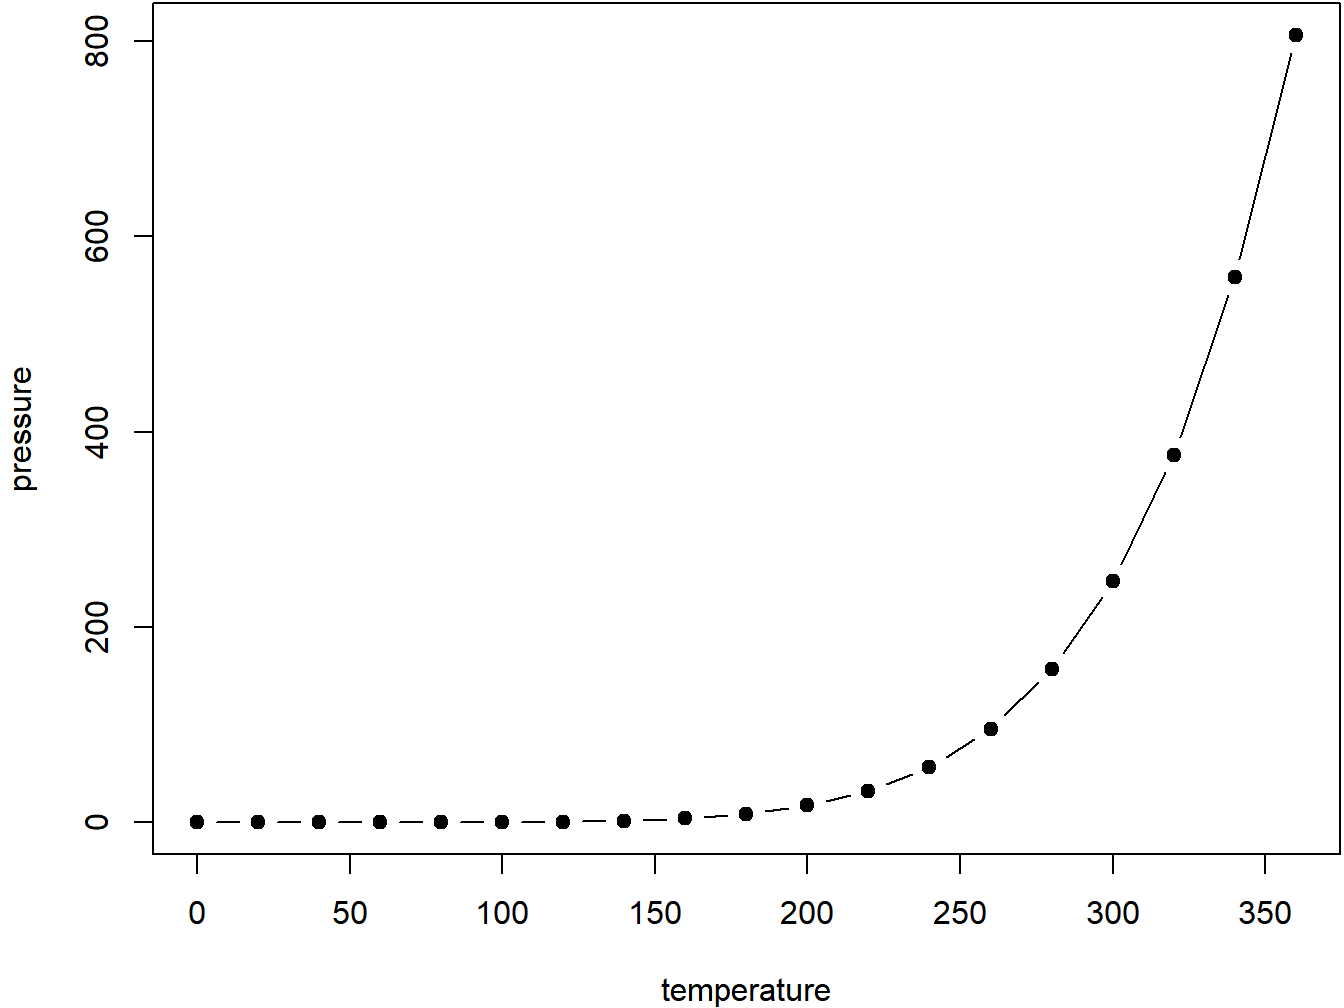
\includegraphics[width=0.8\linewidth]{gitbook-demo_files/figure-latex/nice-fig-1} 

}

\caption{Here is a nice figure!}\label{fig:nice-fig}
\end{figure}

Reference a figure by its code chunk label with the \texttt{fig:} prefix, e.g., see Figure \ref{fig:nice-fig}. Similarly, you can reference tables generated from \texttt{knitr::kable()}, e.g., see Table \ref{tab:nice-tab}.

\begin{Shaded}
\begin{Highlighting}[]
\NormalTok{knitr}\OperatorTok{::}\KeywordTok{kable}\NormalTok{(}
  \KeywordTok{head}\NormalTok{(iris, }\DecValTok{20}\NormalTok{), }\DataTypeTok{caption =} \StringTok{'Here is a nice table!'}\NormalTok{,}
  \DataTypeTok{booktabs =} \OtherTok{TRUE}
\NormalTok{)}
\end{Highlighting}
\end{Shaded}

\label{tab:nice-tab}Here is a nice table!

Sepal.Length

Sepal.Width

Petal.Length

Petal.Width

Species

5.1

3.5

1.4

0.2

setosa

4.9

3.0

1.4

0.2

setosa

4.7

3.2

1.3

0.2

setosa

4.6

3.1

1.5

0.2

setosa

5.0

3.6

1.4

0.2

setosa

5.4

3.9

1.7

0.4

setosa

4.6

3.4

1.4

0.3

setosa

5.0

3.4

1.5

0.2

setosa

4.4

2.9

1.4

0.2

setosa

4.9

3.1

1.5

0.1

setosa

5.4

3.7

1.5

0.2

setosa

4.8

3.4

1.6

0.2

setosa

4.8

3.0

1.4

0.1

setosa

4.3

3.0

1.1

0.1

setosa

5.8

4.0

1.2

0.2

setosa

5.7

4.4

1.5

0.4

setosa

5.4

3.9

1.3

0.4

setosa

5.1

3.5

1.4

0.3

setosa

5.7

3.8

1.7

0.3

setosa

5.1

3.8

1.5

0.3

setosa

You can write citations, too. For example, we are using the \textbf{bookdown} package \citep{R-bookdown} in this sample book, which was built on top of R Markdown and \textbf{knitr} \citep{xie2015}.

\hypertarget{examples}{%
\chapter{Examples}\label{examples}}

Here are some examples of other GitBooks for courses; if you want to have your GitBook added to the list, please send a \href{https://github.com/cjvanlissa/gitbook-demo/pulls}{Pull Request} (here's \href{https://help.github.com/en/github/collaborating-with-issues-and-pull-requests/creating-a-pull-request}{how to send a pull request}).

\hypertarget{doing-meta-analysis-in-r}{%
\section{Doing Meta-Analysis in R}\label{doing-meta-analysis-in-r}}

\url{http://cjvanlissa.github.io/Doing-Meta-Analysis-in-R}

A GitBook on doing meta-analysis in R, based on the book `Doing Meta-Analysis in R', by Mathias Harrer, Pim Cuijpers, \& David Ebert, and adapted to focus on the \href{https://cran.r-project.org/web/packages/metafor/index.html}{metafor} package, and exploring heterogeneity using \href{https://cran.r-project.org/web/packages/metaforest/index.html}{metaforest}. The original can be found here: \url{https://bookdown.org/MathiasHarrer/Doing_Meta_Analysis_in_R/}

\hypertarget{theory-construction-and-statistical-modeling}{%
\section{Theory Construction and Statistical Modeling}\label{theory-construction-and-statistical-modeling}}

\url{http://cjvanlissa.github.io/TCSM}

A GitBook for the course \emph{``Theory Construction and Statistical Modeling''}, with some interesting code, for example: Blocks of answers to the tutorial questions that can be collapsed and expanded.

\hypertarget{open-educational-resources}{%
\chapter{Open Educational Resources}\label{open-educational-resources}}

UNESCO defines Open Educational Resources as \href{https://en.unesco.org/themes/building-knowledge-societies/oer}{\emph{teaching, learning and research materials in any medium -- digital or otherwise -- that reside in the public domain or have been released under an open license that permits no-cost access, use, adaptation and redistribution by others with no or limited restrictions.}}

Open Educational resources can help lighten the workload on individual teachers, who can collaborate with the development of high-quality open access resources, instead of having to develop their own proprietary materials from scratch. Moreover, Open Educational resources are inclusive, lowering the barrier to knowledge acquisition for learners around the world, and enabling lifelong learning for those outside academia.

Many universities support Open Educational Resources. Here are just a few (feel free to \href{https://help.github.com/en/github/collaborating-with-issues-and-pull-requests/creating-a-pull-request}{send a pull request} with other relevant resources).

\begin{itemize}
\tightlist
\item
  \href{https://www.oercommons.org/}{\textbf{OER Commons}}: A freely accessible online library of open educational resources.
\item
  \href{https://uu.figshare.com/}{\textbf{Utrecht University Figshare}}: Open learning objects from Utrecht University.
\item
  \href{https://ocw.jhsph.edu/}{\textbf{Johns Hopkins University OCW}}: Open public health courses and materials.
\item
  \href{https://pitt.libguides.com/openeducation/biglist}{\textbf{University of Pittsburgh OER}}: Big List of Open Educational Resources.
\end{itemize}

\hypertarget{license-your-gitbook}{%
\chapter{License your GitBook}\label{license-your-gitbook}}

In the spirit of Open Science, it is good to think about making your course materials Open Source. That means that other people can use them. In principle, if you publish materials online without license information, you hold the copyright to those materials. If you want them to be Open Source, you must include a license.

The Creative Commons licenses are typically suitable for course materials. This GitBook, for example, is licensed under CC-BY 4.0. That means you can use and remix it as you like, but you must credit the original source.

You can find \href{https://creativecommons.org/share-your-work/licensing-examples}{more information about the Creative Commons Licenses here}. Specific licenses that might be useful are:

\begin{itemize}
\tightlist
\item
  \href{https://creativecommons.org/share-your-work/public-domain/cc0/}{CC0 (``No Rights Reserved'')}, everybody can do what they want with your work
\item
  \href{https://creativecommons.org/licenses/by/4.0/}{CC-BY 4.0 (``Attribution'')}, everybody can do what they want with your work, but they must credit you
\end{itemize}

  \bibliography{book.bib,packages.bib}

\end{document}
